% Options for packages loaded elsewhere
\PassOptionsToPackage{unicode}{hyperref}
\PassOptionsToPackage{hyphens}{url}
\PassOptionsToPackage{dvipsnames,svgnames,x11names}{xcolor}
%
\documentclass[
  12pt,
  a4paper,
]{article}
\usepackage{amsmath,amssymb}
\usepackage{iftex}
\ifPDFTeX
  \usepackage[T1]{fontenc}
  \usepackage[utf8]{inputenc}
  \usepackage{textcomp} % provide euro and other symbols
\else % if luatex or xetex
  \usepackage{unicode-math} % this also loads fontspec
  \defaultfontfeatures{Scale=MatchLowercase}
  \defaultfontfeatures[\rmfamily]{Ligatures=TeX,Scale=1}
\fi
\usepackage{lmodern}
\ifPDFTeX\else
  % xetex/luatex font selection
  \setmainfont[]{Latin Modern Roman}
  \setsansfont[]{Latin Modern Sans}
  \setmonofont[]{Latin Modern Mono}
\fi
% Use upquote if available, for straight quotes in verbatim environments
\IfFileExists{upquote.sty}{\usepackage{upquote}}{}
\IfFileExists{microtype.sty}{% use microtype if available
  \usepackage[]{microtype}
  \UseMicrotypeSet[protrusion]{basicmath} % disable protrusion for tt fonts
}{}
\makeatletter
\@ifundefined{KOMAClassName}{% if non-KOMA class
  \IfFileExists{parskip.sty}{%
    \usepackage{parskip}
  }{% else
    \setlength{\parindent}{0pt}
    \setlength{\parskip}{6pt plus 2pt minus 1pt}}
}{% if KOMA class
  \KOMAoptions{parskip=half}}
\makeatother
\usepackage{xcolor}
\usepackage[top=17mm,bottom=16mm,left=19mm,right=19mm]{geometry}
\usepackage{longtable,booktabs,array}
\usepackage{calc} % for calculating minipage widths
% Correct order of tables after \paragraph or \subparagraph
\usepackage{etoolbox}
\makeatletter
\patchcmd\longtable{\par}{\if@noskipsec\mbox{}\fi\par}{}{}
\makeatother
% Allow footnotes in longtable head/foot
\IfFileExists{footnotehyper.sty}{\usepackage{footnotehyper}}{\usepackage{footnote}}
\makesavenoteenv{longtable}
\setlength{\emergencystretch}{3em} % prevent overfull lines
\providecommand{\tightlist}{%
  \setlength{\itemsep}{0pt}\setlength{\parskip}{0pt}}
\setcounter{secnumdepth}{-\maxdimen} % remove section numbering
\ifLuaTeX
\usepackage[bidi=basic]{babel}
\else
\usepackage[bidi=default]{babel}
\fi
\babelprovide[main,import]{american}
\ifPDFTeX
\else
\babelfont{rm}[]{Latin Modern Roman}
\fi
% get rid of language-specific shorthands (see #6817):
\let\LanguageShortHands\languageshorthands
\def\languageshorthands#1{}
\usepackage{graphicx}
\usepackage{titlesec}
\usepackage{fancyhdr}
\usepackage{xcolor}
\usepackage{array}
\usepackage{microtype}
\usepackage{caption}
\usepackage{fvextra}
\usepackage{etoolbox}
\usepackage{needspace}
\definecolor{navy}{HTML}{0C213B}
\definecolor{sublabel}{HTML}{34536E}
\definecolor{ruleblue}{HTML}{A6B7C7}
\definecolor{bodyink}{HTML}{172330}
\setlength{\parindent}{0pt}
\setlength{\parskip}{5pt plus .8pt minus .3pt}
\setlength{\emergencystretch}{2.6em}
\setlength{\LTpre}{5pt plus 1pt}
\setlength{\LTpost}{5pt plus 1pt}
\setlength{\tabcolsep}{4.5pt}
\renewcommand{\arraystretch}{1.16}
\AtBeginEnvironment{longtable}{\fontsize{9.65pt}{11.7pt}\selectfont}
\AtBeginDocument{\fontsize{10pt}{12.77pt}\selectfont\color{bodyink}}
\titleformat{\section}{\normalfont\fontsize{18bp}{21.5bp}\selectfont\bfseries\color{navy}}{}{0em}{}
\titlespacing*{\section}{0pt}{10pt plus 2pt}{7pt plus 1pt}
\titleformat{\subsection}{\normalfont\fontsize{14.6bp}{18bp}\selectfont\bfseries\color{navy}}{}{0em}{}
\titlespacing*{\subsection}{0pt}{8pt plus 1.5pt}{4.5pt}
\titleformat{\subsubsection}{\normalfont\fontsize{13.3bp}{16.2bp}\selectfont\bfseries\color{navy}}{}{0em}{}
\titlespacing*{\subsubsection}{0pt}{8pt plus 1.5pt}{4pt}
\setlength{\headheight}{23pt}
\setlength{\headsep}{9pt}
\setlength{\footskip}{23pt}
\setlength{\textfloatsep}{10pt plus 3pt minus 2pt}
\setlength{\intextsep}{8pt plus 1.5pt minus 2pt}
\renewcommand{\topfraction}{.87}
\renewcommand{\bottomfraction}{.65}
\renewcommand{\textfraction}{.11}
\renewcommand{\floatpagefraction}{.78}
\setcounter{topnumber}{3}
\setcounter{bottomnumber}{2}
\setcounter{totalnumber}{4}
\captionsetup[figure]{font={footnotesize,color=sublabel},labelfont=bf,labelsep=period,justification=justified,singlelinecheck=false,hypcap=false,skip=4pt}
\newcommand{\parttag}{Main report}
\newcommand{\beginappendix}{\renewcommand{\parttag}{Appendix}}
\newcommand{\notetext}[1]{\par{\fontsize{9.6pt}{11.6pt}\selectfont\itshape\color{sublabel}#1\par}}
\newcommand{\reporttitle}[1]{%
  \pdfbookmark[0]{#1}{report-title}%
  \par\noindent{\raggedright\fontsize{24bp}{26.5bp}\selectfont\bfseries\color{navy}#1\par}\vspace{6pt}}
\newcommand{\deck}[1]{{\raggedright\fontsize{13bp}{16bp}\selectfont\itshape\color{sublabel}#1\par}\vspace{5pt}}
\newcommand{\coursebanner}[2]{\thispagestyle{firstpage}%
  {\fontsize{9.5bp}{12bp}\selectfont\color{sublabel}\textbf{#1}\hfill #2\par}%
  \noindent{\color{ruleblue}\rule{\linewidth}{.65pt}}\par\vspace{8pt}}
\newcommand{\chart}[3]{%
  \par\addvspace{6pt}\noindent
  \begin{minipage}{\linewidth}\centering
    \includegraphics[width=#3\linewidth]{figures/#1.pdf}\par
    \captionof{figure}{#2}%
  \end{minipage}\par\addvspace{6pt}}

\newcommand{\tabletag}[2]{%
  \par\noindent{\fontsize{10.1pt}{11.9pt}\selectfont\bfseries\color{navy}Table #1. #2\par}\nopagebreak[4]}
\newcommand{\chartpair}[3]{%
  \par\addvspace{6pt}\noindent
  \begin{minipage}{\linewidth}\centering
    \includegraphics[width=.52\linewidth]{figures/#1.pdf}\hfill
    \includegraphics[width=.44\linewidth]{figures/#2.pdf}\par
    \captionof{figure}{#3}
  \end{minipage}\par\addvspace{7pt}}
\RecustomVerbatimEnvironment{verbatim}{Verbatim}{breaklines,breakanywhere,fontsize=\small,formatcom=\color{navy},xleftmargin=1em}
\fancyhf{}
\fancyhead[L]{\color{sublabel}\fontsize{9.0bp}{11bp}\selectfont\textbf{BFT65B}\hspace{.85em}Bank Failure Early Warning}
\fancyhead[R]{\color{sublabel}\fontsize{9.0bp}{11bp}\selectfont\parttag}
\fancyfoot[L]{\color{sublabel}\fontsize{8.8bp}{10.5bp}\selectfont National Economics University}
\fancyfoot[R]{\color{navy}\fontsize{9.0bp}{10.5bp}\selectfont\thepage}
\renewcommand{\headrulewidth}{.35pt}
\renewcommand{\headrule}{\hbox to\headwidth{\color{ruleblue}\leaders\hrule height \headrulewidth\hfill}}
\pagestyle{fancy}
\fancypagestyle{firstpage}{\fancyhead{}\renewcommand{\headrulewidth}{0pt}}
\setcounter{secnumdepth}{0}
\widowpenalty=10000
\clubpenalty=10000
\displaywidowpenalty=10000
\raggedbottom
\AtBeginDocument{\hypersetup{pdfauthor={Lê Đức Vượng},pdftitle={A Reproducible Big-Data Pipeline for Bank Failure Early Warning},linkcolor=navy,urlcolor=sublabel}}
\usepackage{multicol}
\setlength{\columnsep}{16pt}
\newcommand{\reflisting}[2]{\par\hangindent=3.0em\hangafter=1\noindent\makebox[3.0em][l]{\textbf{[#1]}}#2\par}
\ifLuaTeX
  \usepackage{selnolig}  % disable illegal ligatures
\fi
\usepackage{bookmark}
\IfFileExists{xurl.sty}{\usepackage{xurl}}{} % add URL line breaks if available
\urlstyle{same}
\hypersetup{
  pdflang={en-US},
  colorlinks=true,
  linkcolor={Maroon},
  filecolor={Maroon},
  citecolor={Blue},
  urlcolor={Blue},
  pdfcreator={LaTeX via pandoc}}

\author{}
\date{}

\begin{document}

\coursebanner{NATIONAL ECONOMICS UNIVERSITY}{BFT65B · Big Data Analytics in Finance}
\reporttitle{A Reproducible Big-Data Pipeline for Bank Failure Early Warning}
\deck{Evidence from FDIC Data and Implications for Vietnam}

\textbf{Student} Lê Đức Vượng · \textbf{Student ID} 11231026 ·
\href{https://github.com/leducvuong8-web/A-Reproducible-Big-Data-Pipeline-for-Bank-Failure-Early-Warning}{GitHub
repository}

\section{Introduction}\label{introduction}

Supervisors need to identify vulnerable banks early enough to
investigate them with limited staff. This report develops a reproducible
pipeline from public FDIC BankFind data to rank four-quarter bank
failure risk and trace each forecast to its reports, features and
decision rule. I devoted considerable time to reconciling the historical
records and documenting analytical decisions so that any remaining
uncertainties are open to constructive review. The analysis examines how
much coverage a quarterly review queue can deliver and draws on the U.S.
evidence to discuss supervisory needs in Vietnam.

\textbf{Acquisition.} The \textbf{23 November 2026} Phase 1 run (UTC)
verified the quarterly Financials cache from the FDIC BankFind API. The
reference snapshots show \textbf{10 November 2026} write dates and
\textbf{15 November 2026} source-retrieval metadata in the matched
cache. Original Financials retrieval dates require the individual
quarter manifests.

\begingroup
\fontsize{9.4bp}{12bp}\selectfont
\setlength{\tabcolsep}{2.2pt}
\noindent
\begin{minipage}[t]{.422\linewidth}
\raggedright\textbf{Table 1a. FDIC source archives}\par\smallskip
\begin{tabular*}{\linewidth}{@{\extracolsep{\fill}}llr@{}}
\toprule
Archive & Coverage & Rows\\
\midrule
Financials & 1984Q1--2026Q2 & 1,682,616\\
Failures & Events and assistance & 4,117\\
Institutions & Institution history & 27,835\\
\bottomrule
\end{tabular*}
\end{minipage}\hfill
\begin{minipage}[t]{.551\linewidth}
\raggedright\textbf{Table 1b. Forecast windows}\par\smallskip
\begin{tabular*}{\linewidth}{@{\extracolsep{\fill}}llrrr@{}}
\toprule
Window & Origins & Rows & Pos. qtrs & Failures\\
\midrule
Development & 1985Q1--2006Q4 & 1,121,901 & 8,239 & 2,228\\
Crisis test & 2008Q1--2012Q4 & 157,851 & 1,880 & 465\\
Recent OOT & 2014Q1--2025Q2 & 249,606 & 175 & 56\\
\bottomrule
\end{tabular*}
\end{minipage}\par
\endgroup

\notetext{Positive quarters count eligible origins followed by failure within four quarters (Phase 5). Failures count registry events dated inside each window (Phase 2). Both 2025 failures occurred by June.}

The evidence addresses three questions about storing and processing the
reports, constructing a defensible target and applying the model under
limited review capacity.

\textbf{Q1.} How can a laptop store and process forty years of reports,
and when would Spark scale-out help?\\
\textbf{Q2.} What defects affect the panel, and how can I handle exits
and avoid look-ahead?\\
\textbf{Q3.} Can the pipeline support a validated early-warning model
and a feasible review queue?

\textbf{Five implementation phases.} Phase 1 acquires and stores data
after the Phase 0 field audit. Phase 2 checks quality and constructs the
panel and labels. Phase 3 tests Polars, pandas and PySpark
transformations. Phase 4 engineers features and joins labels. Phase 5
fits, validates and evaluates the models.

\textbf{Answers in brief.} For Q1, Snappy Parquet reduced stored size by
\textbf{47.99\%} across five benchmark years. On matching 2024 features,
Polars, pandas and local Spark took \textbf{120.65, 155.20 and 1,686.02
ms} at the median. For Q2, I used calendar-exact histories, separate
exit reasons and a mature four-quarter label. A prior-quarter OOF score
proxy illustrates the operational cost of delayed information. For Q3,
recency-weighted RF achieves \textbf{AP 0.63361} and \textbf{278/487}
banks detected in Crisis at Top 25 per quarter. In Recent OOT, it
reaches \textbf{AP 0.37201} and \textbf{44/53} banks. Precision and
recall track correct alert rows, bank recall tracks institutional
coverage, and false alerts and Brier score measure review burden and
probability error.

\textbf{What is independently checked.} Source completeness is verified
against API totals and bank--quarter keys. Feature validity is checked
with independent implementations and forecasts that respect exact
calendar gaps. Model comparisons pair the same development rows and use
equal review capacity. This lets a reviewer trace a result back to the
underlying data and isolate whether a difference came from the source, a
transformation or the alarm policy.

\newpage
\setlength{\parskip}{2.9pt plus .55pt minus .3pt}
\renewcommand{\arraystretch}{1.10}
\fontsize{10pt}{12.77pt}\selectfont

\section{1. Data Acquisition and
Storage}\label{data-acquisition-and-storage}

\subsection{1.1 API extraction, resumption and
completeness}\label{api-extraction-resumption-and-completeness}

The archived acquisition contract covers 136 fields from a catalogue of
2,378 documented fields {[}1{]}. The contract contains the two keys and
the inputs that support capital, loan quality, earnings and funding
measures. An overlap audit flagged 86 field pairs for review. For
example, total deposits and domestic deposits differ in coverage. I
compared definitions, units and values before treating fields as
substitutes.

\textbf{Phase 0 literature review.} The research matrix contains exactly
26 entries {[}R01--R26{]}. The concept extraction produces 63
source-to-concept links, retaining study IDs, links and matched
predictor phrases. These associations support candidate risk mechanisms
and raw-field requirements. The archived 136-field acquisition contract
is the source of the measured pipeline results. Section 4.1.1 documents
the separately dated rationale and the development-only model selection
protocol.

\texttt{quarter\_extract} translates a quarter into its reporting date,
divides the fields into batches and calls \texttt{fetch\_pages}. Each
batch carries CERT and REPDTE. It validates dates, unique keys, API
totals and identical key sets before a one-to-one merge. A field omitted
because all values are missing is restored as null. The collector sorts
the stitched result and verifies the count before writing. Using key
sets catches the case where one bank disappears and another replaces it
while the row count stays the same.

\tabletag{2}{Expected scope, observed scope and verification}

\begin{longtable}[]{@{}
  >{\raggedright\arraybackslash}p{(\columnwidth - 4\tabcolsep) * \real{0.3333}}
  >{\raggedright\arraybackslash}p{(\columnwidth - 4\tabcolsep) * \real{0.3333}}
  >{\raggedright\arraybackslash}p{(\columnwidth - 4\tabcolsep) * \real{0.3333}}@{}}
\toprule\noalign{}
\begin{minipage}[b]{\linewidth}\raggedright
Expected scope
\end{minipage} & \begin{minipage}[b]{\linewidth}\raggedright
Observed scope
\end{minipage} & \begin{minipage}[b]{\linewidth}\raggedright
Validation
\end{minipage} \\
\midrule\noalign{}
\endhead
\bottomrule\noalign{}
\endlastfoot
170 quarters, 1984Q1--2026Q2 & 170 quarters, 1,682,616 rows & API totals
and stitched quarterly keys reconciled \\
Historical failure and assistance records & 4,117 rows & Independent
event snapshot verified for Phase 2 \\
Institution reference & 27,835 rows & Separate identity and exit
reference \\
Annual Bronze output & 43 files, 136 fields & Raw values reconciled
after typing and regrouping \\
Technical acquisition controls & 12/12 passed & Archived output accepted
against the field contract \\
\end{longtable}

\notetext{Source: Phase 0 §§9.5–9.7 and Phase 1 §§2–5, 9. Financials contains 24,064 distinct CERTs. 2026 is a partial year.}

\textbf{Recovery.} \texttt{acquire\_quarter} checks the Raw
file--manifest pair. \texttt{verify\_raw} validates SHA-256, schema,
date, unique keys and row count. A new quarter is staged and checked
before promotion. An incomplete pair causes an explicit failure for
review. The failure snapshot has tied event dates, so if its response
needs splitting, the collector can partition by year and validate each
total.

\textbf{Acquisition metadata (§2.2A).} All six checks reach 170/170: Raw
files, manifests, recorded SHA-256 digests, matching field contracts,
retrieval timestamps and file-write timestamps. All 8,835 logged legacy
API pages have zero retained page digests and zero page retrieval
timestamps. The archival snapshots and quarterly evidence are preserved.
Acquisition timestamps date retrieval and storage. Verified bank-report
publication dates require separate evidence. Appendix A distinguishes an
API refresh from an exact replay.

\textbf{Failure injection before the full extraction.} Phase 1 §0.2 uses
synthetic API responses to exercise the same page and manifest checks as
acquisition. It rejects duplicate pages and nonmonotone key order. A
separate one-byte alteration to a pinned input triggers the digest gate.
The three tests passed. An identical total alone would miss a duplicated
bank and an omitted bank, so the collector checks both the row total and
the ordered identity keys.

\subsubsection{1.1.1 What makes a quarterly download
reproducible}\label{what-makes-a-quarterly-download-reproducible}

The versioned field contract controls acquisition. Its digest changes
when a field is added or removed. I preserve that identity in the
quarter manifest along with the requested quarter-end, selected names,
page records, row count and content digest. The hash answers whether I
opened the original result. The expected date and distinct keys identify
the intended quarter. Downloading current data and reproducing a
historical run are therefore separate operations.

\subsection{1.2 Schema, partitioning and measured
trade-offs}\label{schema-partitioning-and-measured-trade-offs}

I retain stitched API values as strings in quarterly Raw Parquet, then
apply explicit types with \texttt{typecast\_raw\_table}. Bronze uses
integer CERT, Date32 REPDTE and Float64 for source fields that may
contain integers and decimals. Source nulls are preserved. A value that
cannot be converted is surfaced for inspection. Bronze is partitioned by
year and uses Snappy. The engineered W1 output uses ZSTD.

I wrote the same Arrow table as CSV, Parquet Snappy and Parquet ZSTD and
measured each in randomized order across seven repetitions per year and
format. The read benchmark materializes CERT, REPDTE, ASSET, DEP and EQ.
File-size savings aggregate bytes across years before dividing. A cold
cache was not isolated in the cited experiment.

\tabletag{3}{Matched storage and projection benchmark for 2024}

\begin{longtable}[]{@{}lrrr@{}}
\toprule\noalign{}
Format & Size (MiB) & Five-column read (ms) & Write median (ms) \\
\midrule\noalign{}
\endhead
\bottomrule\noalign{}
\endlastfoot
CSV & 10.425 & 8.943 & 196.413 \\
Parquet Snappy & 6.364 & 2.096 & 141.639 \\
Parquet ZSTD & 5.068 & 2.178 & 154.158 \\
\end{longtable}

\notetext{Source: Phase 1 §§6.3–6.5. Each format contains the same 18,399 rows and 136 fields.}

\chart{storage_projection}{Five-column projection latency across five measured years. Source: Phase 1 §6.5.}{.66}

Across the benchmark years, Snappy and ZSTD saved \textbf{47.99\%} and
\textbf{57.01\%} relative to CSV. In 2024, the respective projection
reads were about 4.27× and 4.11× as fast. Parquet can skip unrequested
column chunks. The measured benefit applies to this workload and file
layout. The two Parquet codecs differ by just 0.082 ms in the 2024 read.

\textbf{Why partition by year?} The 2024 Q1-only read took 1.305 ms from
a quarterly partition and 3.976 ms from the annual file. Quarterly
partitions consumed 10.24--13.84\% more space in the experiment. I keep
quarter-level recovery upstream and annual Bronze for workloads that
repeatedly scan multiple quarters. A service centered on one-quarter
reads can benchmark a separate quarterly serving copy with its lookback
included. Appendix A reports the per-year results.

Phase 1 uses a retry budget of five on rate-limit and selected server
errors, with backoff and support for the server's retry delay. Its
separate Raw-to-Bronze check retypes the quarterly files and compares
every persisted cell across all 43 annual files. This validates the
storage transformation in addition to verifying the bytes of each file.

\section{2. Data Quality and Bank--Quarter
Panel}\label{data-quality-and-bankquarter-panel}

\subsection{2.1 Automated audit and defect
resolution}\label{automated-audit-and-defect-resolution}

\texttt{export\_silver} reads annual Bronze, applies
\texttt{add\_quality\_columns}, writes row groups and reads the result
back to check source columns and keys. I keep the original financial
value and attach flags. Negative equity can signal distress. An extreme
asset change may indicate restructuring, consolidation changes or a
source error. For both cases, I check adjacent reports and institution
evidence before drawing a financial conclusion.

\Needspace{8\baselineskip}

\tabletag{4}{Observed issues and audit response}

\begin{longtable}[]{@{}
  >{\raggedright\arraybackslash}p{(\columnwidth - 4\tabcolsep) * \real{0.3333}}
  >{\raggedright\arraybackslash}p{(\columnwidth - 4\tabcolsep) * \real{0.3333}}
  >{\raggedright\arraybackslash}p{(\columnwidth - 4\tabcolsep) * \real{0.3333}}@{}}
\toprule\noalign{}
\begin{minipage}[b]{\linewidth}\raggedright
Issue
\end{minipage} & \begin{minipage}[b]{\linewidth}\raggedright
Observed scope
\end{minipage} & \begin{minipage}[b]{\linewidth}\raggedright
Response and verification
\end{minipage} \\
\midrule\noalign{}
\endhead
\bottomrule\noalign{}
\endlastfoot
Unlinked institution records & 234 CERTs in the audited exit subset &
Check institutional and event evidence before resolving the exit \\
Unexplained report cessation & 70,901 bank--quarters in the initial
diagnostic & Record distinct outcome branches and retain the stricter
sensitivity cohort \\
Event identity or date ambiguity & 488 rows without CERT and 6 with
conflicting failure dates & Quarantine before automatic event linking \\
Financial field semantics & 134 definitions in the expanded audit still
need independent certification & Preserve nulls and screen field
availability within training windows \\
Publication time & 1,096 candidate positives differ under the 0- and
45-day scenarios & Record sensitivity and require receipt history for
operational replay \\
\end{longtable}

\notetext{Source: Phase 2 cells 308 and 379–381. Each issue has its own denominator.}

\chart{historical_coverage}{Completeness of six core fields by row and availability of 133 financial fields by cell. Source: Phase 2 §2.6.4A.}{.61}

\textbf{Result and decision.} \texttt{deep\_quality\_gate\_table} passed
\textbf{20/20} consistency checks for coverage, keys, lineage and
events. For 1984--1994, 97.74\% of rows had all six core fields, while
67.73\% of the 133-field cells were available. By 2005--2025Q2 these
rates reached 99.71\% and 89.09\%. In a separate era check, RBCT1C was
absent in 2005--2009 and nearly universal in 2017--2025Q2. Filling a
structurally unavailable capital field with zero would create a
misleading financial value. I retain nulls and make preprocessing
decisions inside each training fold. Appendix B documents the audit
boundaries.

\subsubsection{2.1.1 Distinguish source values, derived values and
unknown
outcomes}\label{distinguish-source-values-derived-values-and-unknown-outcomes}

A blank source value stays null with its reporting context. A field
missing after calculation can indicate an unavailable calendar anchor or
an invalid denominator. A missing target indicates an unresolved or
immature outcome. Imputing a predictor inside a training fold may be
appropriate. Imputing a target alters the set of outcomes on which the
model is judged. This also explains why the rate of missing labels
should be read separately from financial-field coverage.

\subsubsection{2.1.2 What changed at the 2016Q4--2017Q1
boundary}\label{what-changed-at-the-2016q42017q1-boundary}

Phase 2 §2.5.3 matched 5,923 of the 5,925 banks reporting at 2017Q1 to
an actual 2016Q4 record. Reconstructing quarter-on-quarter transitions
raised the modern sample's count of asset increases above 100\% from 147
to 150 and contractions beyond 50\% from 31 to 32. Each of the four new
flags reconciled to a valid historical pair. Across five boundary
quarters the same check matched 25,167 observations and all 136 source
fields. The independent full-panel check (§2.5.5) passed all 5,848
year-by-field comparisons, with 1,682,616 rows on each side.

\Needspace{8\baselineskip}

\tabletag{4a}{Effect of four missing-ROE policies on 172,924 bank–quarters}

\begin{longtable}[]{@{}
  >{\raggedright\arraybackslash}p{(\columnwidth - 8\tabcolsep) * \real{0.2000}}
  >{\raggedleft\arraybackslash}p{(\columnwidth - 8\tabcolsep) * \real{0.2000}}
  >{\raggedleft\arraybackslash}p{(\columnwidth - 8\tabcolsep) * \real{0.2000}}
  >{\raggedleft\arraybackslash}p{(\columnwidth - 8\tabcolsep) * \real{0.2000}}
  >{\raggedleft\arraybackslash}p{(\columnwidth - 8\tabcolsep) * \real{0.2000}}@{}}
\toprule\noalign{}
\begin{minipage}[b]{\linewidth}\raggedright
Policy
\end{minipage} & \begin{minipage}[b]{\linewidth}\raggedleft
Rows removed
\end{minipage} & \begin{minipage}[b]{\linewidth}\raggedleft
Hypothetical fills
\end{minipage} & \begin{minipage}[b]{\linewidth}\raggedleft
Missing ROE left
\end{minipage} & \begin{minipage}[b]{\linewidth}\raggedleft
Negative-equity rows retained
\end{minipage} \\
\midrule\noalign{}
\endhead
\bottomrule\noalign{}
\endlastfoot
Preserve nulls & 0 & 0 & 717 & 207 \\
Complete cases & 717 & 0 & 0 & 84 \\
Training-median candidate & 0 & 139 & 578 & 207 \\
Exact prior-quarter ROE candidate & 0 & 22 & 695 & 207 \\
\end{longtable}

\notetext{Source: Phase 2, cell 133. The fill counts assess eligibility under alternative rules. Silver values are preserved.}

Complete-case deletion removes 123 of 207 negative-equity rows (59.4\%).
In 17 of the 22 lag-fill candidates, current equity is negative and
prior-quarter ROE is positive. The median rule would fill ROE for 123
negative-equity rows. These results explain why Silver preserves nulls
and the equity flag, leaving any feature imputation to the training
pipeline.

\textbf{Auditing the cost of aggressive cleaning.} Phase 2 §4.4 compares
complete-case deletion and annual tail clipping against the preserved
source. In the full-history audit, 15,659 rows from 2,837 banks have
negative equity. The transition review associates 10,439 classifications
with negative earnings and 3,055 with capital recovery while equity
remains negative. These categories are diagnostics from observed
histories. Silver retains the numerical signs and flags so a later
training fold can distinguish a missing field from an observed value at
the tail. Phase 2 also reconciles 33 internal gap episodes across 32
banks to 92 missing quarters in its continuity audit. Missing
intermediate reports remain absent, so growth and rolling features must
use exact date arithmetic.

\subsection{2.2 One row per bank--quarter and competing
exits}\label{one-row-per-bankquarter-and-competing-exits}

\textbf{Identifier verification.} Phase 2 §2.1.8A shows that an integer
cast of the string \texttt{14571.0} produces null and can silently miss
a match. The normalized bank and event sets reconcile independently to
\textbf{3,241 common CERTs}. This is a broad linkage audit. The final
registry enforces event dates, distinguishes failure and assistance, and
quarantines ambiguous records before the many-to-one join to unique
bank--quarter rows.

\tabletag{5}{Panel disposition and consequence for modelling}

\begin{longtable}[]{@{}
  >{\raggedright\arraybackslash}p{(\columnwidth - 4\tabcolsep) * \real{0.3333}}
  >{\raggedright\arraybackslash}p{(\columnwidth - 4\tabcolsep) * \real{0.3333}}
  >{\raggedright\arraybackslash}p{(\columnwidth - 4\tabcolsep) * \real{0.3333}}@{}}
\toprule\noalign{}
\begin{minipage}[b]{\linewidth}\raggedright
Evidence
\end{minipage} & \begin{minipage}[b]{\linewidth}\raggedright
Audit status
\end{minipage} & \begin{minipage}[b]{\linewidth}\raggedright
Model consequence
\end{minipage} \\
\midrule\noalign{}
\endhead
\bottomrule\noalign{}
\endlastfoot
Verified failure in the next four quarters & Dated failure & Positive if
the forecast row is eligible \\
Merger or competing closure & Distinct exit reason & No qualifying
failure gives 0 if the registry horizon is mature \\
Assistance & Separate event type & Does not satisfy the failure
definition \\
Unresolved administrative exit & High-risk review flag & V3 event rule
for the main cohort, excluded from strict sensitivity \\
Incomplete event follow-up & Right-censored & Unavailable for binary
evaluation \\
Pre-existing or conflicting failure & Exclusion or quarantine & Retained
in audit only \\
\end{longtable}

\chart{label_resolution}{How the V3 event rule resolves previously missing V2 labels. Source: Phase 2 cells 412–418.}{.66}

The FDIC History supplement contains \textbf{508,660 source-ID-unique
records} across \textbf{32,340 CERTs}, with SHA verification in Phase 2
§5.1. It adds dated change codes for the competing-event review.
Verified history accounts for 55,754 merger bank--quarters and 1,714
closure bank--quarters. Evidence for the event type, its date and the
maturity of the registry horizon govern whether a record remains unknown
or enters V3 as an eligible negative.

The \textbf{7,514} unresolved administrative exits affect \textbf{2,059
banks}. They retain a review flag. An eligible zero means no qualifying
failure in the mature registry window. Appendix B quantifies how the
strict V3 filter changes cohort sizes.

\textbf{Why competing exits matter.} Oshinsky and Olin {[}R07{]} study
recoveries, mergers and failures among troubled institutions. Wheelock
and Wilson {[}H15{]} model acquisition and failure as competing events
in 1984--1993. Lane et al.~{[}H14{]} and Whalen {[}H10{]} illustrate
time-to-event alternatives. I use a fixed four-quarter target and retain
the competing-event flags even when the eligible label is zero.

\subsection{2.3 Four-quarter target, cutoff and
availability}\label{four-quarter-target-cutoff-and-availability}

For bank \(i\) at quarter-end \(q\), let \(F_i\) denote a qualifying
FDIC failure date. On eligible bank--quarters I define \[
y_{i,q}=\mathbf{1}\{q<F_i\leq q+4\text{ calendar quarters}\}.
\]

\chart{label_timeline}{Example with a 2020Q4 forecast origin. A qualifying event at the 2021Q4 end is included. An event at the origin or beyond the upper boundary is excluded.}{.78}

The construction sets the exact fourth quarter-end. It compares that
date with the event-source availability date and checks the valid risk
set. A row enters \texttt{MODEL\_ELIGIBLE\_V3} with a known target, a
mature event horizon and an observed, valid origin. The assignment
additionally caps origins at \textbf{30 June 2025}. Later registry
outcomes can mature earlier forecasts without entering predictors.

\tabletag{6}{V2-to-V3 reconciliation and eligibility}

\begin{longtable}[]{@{}
  >{\raggedright\arraybackslash}p{(\columnwidth - 4\tabcolsep) * \real{0.3333}}
  >{\raggedleft\arraybackslash}p{(\columnwidth - 4\tabcolsep) * \real{0.3333}}
  >{\raggedright\arraybackslash}p{(\columnwidth - 4\tabcolsep) * \real{0.3333}}@{}}
\toprule\noalign{}
\begin{minipage}[b]{\linewidth}\raggedright
Audit quantity
\end{minipage} & \begin{minipage}[b]{\linewidth}\raggedleft
Count
\end{minipage} & \begin{minipage}[b]{\linewidth}\raggedright
Meaning
\end{minipage} \\
\midrule\noalign{}
\endhead
\bottomrule\noalign{}
\endlastfoot
Missing V2 targets & 85,791 & Starting set of unresolved rows \\
Resolved to zero in V3 & 71,475 & Mature windows under the event rule \\
Still missing & 14,316 & 13,070 right censored, 1,176 pre-existing, 70
quarantined \\
V3 main / strict eligible & 1,668,293 / 1,660,779 & Full audit before W1
and split filters \\
\end{longtable}

\notetext{Source: Phase 2 cells 412–418. The stricter cohort drops 7,514 flagged administrative rows.}

\textbf{Three denominators.} Crisis contains \textbf{465 dated
failures}, above the assignment minimum of 50 {[}3, 4{]}. The archived
scorecard has 1,880 positive forecast quarters for 487 banks. One
failure can make several origins positive, and a late-2012 report can
predict a 2013 event. I use the dated count to describe Crisis coverage
and the 487 positive banks as the bank-recall denominator. Appendix B
shows the annual event chronology.

\subsubsection{2.3.1 Separate outcome follow-up from feature
availability}\label{separate-outcome-follow-up-from-feature-availability}

\textbf{Two data cutoffs.} Phase 2 uses 30 June 2026 as the financial
panel end and 15 November 2026 as the event snapshot date. The last
scored origin, 30 June 2025, needs outcome follow-up through 30 June
2026. Later events and institution changes support the eligibility and
outcome audit. A predictor allowlist excludes failure dates, activity
and termination fields, change codes, maturity flags and censoring
reasons.

\textbf{Operational timing audit.} Cell 387 exports
\texttt{availability\_policy.json} and a keyed
\texttt{availability\_sensitivity\_audit.parquet}. It sets an
illustrative decision date at quarter-end plus 45 calendar days, builds
availability flags under lags of 0, 30, 45 and 90 days, and records the
preceding quarter-end as the conservative feature proxy. A report for 30
June 1984 would reach its assumed 45-day release date on 14 August.
Under the 90-day scenario its release would fall on 28 September,
outside that decision date. The lag exercise and the assignment label
use the same fourth-quarter horizon. Failures by the assumed release
date fall outside the decision-time risk set.

\tabletag{6a}{Candidate positives under hypothetical availability lags}

\begin{longtable}[]{@{}
  >{\raggedright\arraybackslash}p{(\columnwidth - 10\tabcolsep) * \real{0.1667}}
  >{\raggedleft\arraybackslash}p{(\columnwidth - 10\tabcolsep) * \real{0.1667}}
  >{\raggedleft\arraybackslash}p{(\columnwidth - 10\tabcolsep) * \real{0.1667}}
  >{\raggedleft\arraybackslash}p{(\columnwidth - 10\tabcolsep) * \real{0.1667}}
  >{\raggedleft\arraybackslash}p{(\columnwidth - 10\tabcolsep) * \real{0.1667}}
  >{\raggedleft\arraybackslash}p{(\columnwidth - 10\tabcolsep) * \real{0.1667}}@{}}
\toprule\noalign{}
\begin{minipage}[b]{\linewidth}\raggedright
Lag after quarter-end (days)
\end{minipage} & \begin{minipage}[b]{\linewidth}\raggedleft
0
\end{minipage} & \begin{minipage}[b]{\linewidth}\raggedleft
30
\end{minipage} & \begin{minipage}[b]{\linewidth}\raggedleft
45
\end{minipage} & \begin{minipage}[b]{\linewidth}\raggedleft
60
\end{minipage} & \begin{minipage}[b]{\linewidth}\raggedleft
90
\end{minipage} \\
\midrule\noalign{}
\endhead
\bottomrule\noalign{}
\endlastfoot
Candidate positive bank--quarters & 10,859 & 10,172 & 9,763 & 9,383 &
8,371 \\
\end{longtable}

\notetext{Source: Phase 2 cell 372, full-history lag diagnostic. Lag 45 removes 1,096 candidates relative to lag 0.}

\textbf{Verification boundary.} Cell 374 validates an optional
SHA-pinned release file and reports zero supplied timestamps in the
archived run. Phase 5 uses the assignment's quarter-end V3 target. A
development-only proxy replay would map each decision to the exact
preceding report quarter, preserve a null when that report is absent,
and tabulate scoreable rows and eligible events. A vintage replay
additionally needs verified release times and dated versions, and would
select only values public by the decision date.

On development OOF only, Strict V3 excludes 2,271 uncertain
administrative-exit observations with no positive labels removed. This
subset is distinct from the 7,514 observations across 2,059 banks in the
full Main V3 audit. Section 5.2 reports the label and prior-quarter
score sensitivities alongside the Phase 2 availability scenarios.

\section{3. Scalable Processing with Polars and
PySpark}\label{scalable-processing-with-polars-and-pyspark}

\textbf{Environment audit (§3.0.1A).} The audited machine uses an Intel
CPU with 12 physical and 16 logical cores, 15.69 GiB RAM (1.96 GiB
available at audit), Windows 11 AMD64, Python 3.13.7, pandas 2.3.3,
Polars 2.1.0 and NumPy 2.3.3. Polars reports 16 threads. The
configuration specifies one warm-up and three measured repetitions. This
snapshot documents the audit environment. Historical benchmarks retain
their recorded scope, and the evidence supports single-machine
comparisons.

\subsection{3.1 Architecture and measured
workloads}\label{architecture-and-measured-workloads}

\chart{pipeline_architecture}{Stages and verified volumes. Silver preserves financial values and sends outcomes through a separate keyed product. Sources: Phases 1–5.}{.79}

I retain separate products for raw reports, typed financial history,
outcomes, features and a scoring release. This lets an investigator
change an exit rule without changing the financial archive. Phase 3
reads Silver history to calculate W1 using only financial predictors.
Phase 4 joins V3 labels to W1 on the validated key. A matched key and an
eligible outcome are different checks.

\tabletag{7}{Interfaces and phase outputs}

\begin{longtable}[]{@{}
  >{\raggedright\arraybackslash}p{(\columnwidth - 4\tabcolsep) * \real{0.3333}}
  >{\raggedright\arraybackslash}p{(\columnwidth - 4\tabcolsep) * \real{0.3333}}
  >{\raggedright\arraybackslash}p{(\columnwidth - 4\tabcolsep) * \real{0.3333}}@{}}
\toprule\noalign{}
\begin{minipage}[b]{\linewidth}\raggedright
Stage
\end{minipage} & \begin{minipage}[b]{\linewidth}\raggedright
Code or product
\end{minipage} & \begin{minipage}[b]{\linewidth}\raggedright
Archived release evidence
\end{minipage} \\
\midrule\noalign{}
\endhead
\bottomrule\noalign{}
\endlastfoot
Phase 0--1 & Field contract and annual Bronze & 170 quarters, verified
source recovery \\
Phase 2 & Silver and keyed label V3 & Stable raw values with separate
quality and outcome flags \\
Phase 3 & W1 with nine core features & 1,610,856 keyed feature rows \\
Phase 4 & Gold and manifest & Zero W1 keys without a corresponding label
record \\
Phase 5 & Fitted pipeline and frozen specification & Ordered predictors,
calibration, threshold and review policy \\
\end{longtable}

\subsubsection{3.1.1 Narrow and Wide under the same timed
action}\label{narrow-and-wide-under-the-same-timed-action}

A separate Phase 3 low-memory notebook processes 1,682,616 Silver rows
from 24,064 institutions. Narrow reads 11 inputs and writes 20 columns,
including nine derived fields. Wide reads 135 inputs and writes 5,719
year-by-field summaries across 43 years and 133 financial fields, each
with six statistics. Narrow maintains one output per bank--quarter and
needs ordered histories. Wide uses grouped reductions and operates on
many fields at once.

\tabletag{7a}{Full-panel benchmark, medians of five source-to-output runs}

\begin{longtable}[]{@{}
  >{\raggedright\arraybackslash}p{(\columnwidth - 6\tabcolsep) * \real{0.2500}}
  >{\raggedleft\arraybackslash}p{(\columnwidth - 6\tabcolsep) * \real{0.2500}}
  >{\raggedleft\arraybackslash}p{(\columnwidth - 6\tabcolsep) * \real{0.2500}}
  >{\raggedleft\arraybackslash}p{(\columnwidth - 6\tabcolsep) * \real{0.2500}}@{}}
\toprule\noalign{}
\begin{minipage}[b]{\linewidth}\raggedright
Local engine
\end{minipage} & \begin{minipage}[b]{\linewidth}\raggedleft
Narrow seconds
\end{minipage} & \begin{minipage}[b]{\linewidth}\raggedleft
Wide seconds
\end{minipage} & \begin{minipage}[b]{\linewidth}\raggedleft
Narrow / Wide process RSS (MiB)
\end{minipage} \\
\midrule\noalign{}
\endhead
\bottomrule\noalign{}
\endlastfoot
pandas & 18.024 & 28.864 & 3,658 / 5,679 \\
Polars Lazy & 2.568 & 3.240 & 3,021 / 6,009 \\
Spark Local & 68.315 & 81.616 & 4,362 / 5,899 \\
\end{longtable}

\notetext{Source: Phase 3 low-memory §§3.6.4–3.7.3. Median sampled peak RSS is from the benchmark monitor. The numbers describe local processes and cannot be read as distributed executor memory.}

The benchmark forces the output action after one excluded warm-up and
deletes its transient file after each run. Full-key comparison found
zero mismatches across the 18 numeric Narrow fields and zero across
34,314 Wide statistics for each engine comparison. Maximum finite-mean
difference for Spark Wide was \(4.66\times10^{-10}\). These checks
establish full-panel parity for this notebook's contracts. The aligned
W1 benchmark in §3.3 uses a different feature contract, lookback and
output action, so its timings answer a separate question.

\textbf{Scale versus memory.} For these full-panel runs, Polars is
approximately 7.0 times faster than pandas on Narrow and 8.9 times
faster on Wide. Wide Polars peak RSS is \textbf{6,009 MiB}, 330 MiB
above pandas. The Wide workload keeps more field-level aggregation
state, so the faster engine can still hit a memory budget as columns
increase. I track wall time and RSS together when selecting a workload
implementation.

\subsection{3.2 Polars implementation and execution
plan}\label{polars-implementation-and-execution-plan}

\texttt{p3\_w1\_window} scans Parquet lazily, selects 11 input columns
for nine features, creates a calendar index and sorts by institution and
date. It computes shifts within CERT. \texttt{p3\_quarter\_lag} accepts
a shifted value only at the exact requested calendar gap. I implemented
a four-join W1 path and an independent pandas version to verify the same
output.

\tabletag{8}{Condensed optimized Polars plan}

\begin{verbatim}
FILTER REPDTE >= 2024-01-01             output boundary
  WITH_COLUMNS [lags and finite-value checks]
    SORT BY CERT, REPDTE                 ordered bank windows
      FILTER REPDTE between 2023-01-01 and 2024-12-31
        Parquet SCAN [canonical Silver]
        PROJECT 11/141 COLUMNS
\end{verbatim}

The plan shows scan-level projection of 11 of 141 columns. A source-date
interval provides the historical inputs, while a later filter keeps only
the requested output. The archived W1 collector uses streaming with
predicate pushdown disabled to preserve the tested lookback boundary. I
therefore treat the scan-only predicate experiment as separate evidence
about filter syntax.

\begin{longtable}[]{@{}
  >{\raggedright\arraybackslash}p{(\columnwidth - 4\tabcolsep) * \real{0.3333}}
  >{\raggedright\arraybackslash}p{(\columnwidth - 4\tabcolsep) * \real{0.3333}}
  >{\raggedright\arraybackslash}p{(\columnwidth - 4\tabcolsep) * \real{0.3333}}@{}}
\toprule\noalign{}
\begin{minipage}[b]{\linewidth}\raggedright
Experiment
\end{minipage} & \begin{minipage}[b]{\linewidth}\raggedright
Observed median
\end{minipage} & \begin{minipage}[b]{\linewidth}\raggedright
Decision
\end{minipage} \\
\midrule\noalign{}
\endhead
\bottomrule\noalign{}
\endlastfoot
Scan projection & 3.50 ms for 11 fields, 13.24 ms for 141 fields &
Select only the inputs W1 needs \\
Date-filter formulation & Direct range 3.22 ms, extracted year 48.68 ms
& Use a direct bound in scan-only tasks and inspect the plan \\
W1 execution engine & Streaming 101.551 ms, in-memory 84.526 ms & Both
passed parity. Choose using measured latency and memory \\
\end{longtable}

\notetext{Source: Phase 3 §§3.7 and 3.9.2. These timings refer to separate measured tasks.}

The join-based path creates shifted lookup branches. The grouped-window
path uses shifts and a calendar check within each bank. A sort is
required if source order is unverified. For an annual quality report, a
group-by reduces the data to one row per year. The feature computation
instead preserves the panel rows.

On 188 sampled rows I tested changes to future values, permuted order
and truncated input after the evaluation boundary. All three invariance
checks passed. Additional edge cases exercise missing quarters and
invalid numeric values. The checked plan and these tests show why
trimming the output too early would change the calculation. Appendix C
records the reproducible parity method.

\textbf{Calendar checks for missing quarters.} If a bank has Q1, Q3 and
Q4 observations, a previous-row lookup for Q3 would return Q1. The
calendar-index check rejects that value as a one-quarter lag because the
indices differ by two. The same check prevents a four-observation
rolling window from silently spanning five quarters. Surviving the
shuffle and future-data tests establishes temporal consistency of the
calculation across input order and date boundaries.

\subsection{3.3 Matched benchmark against
pandas}\label{matched-benchmark-against-pandas}

I measured pandas, Polars lazy and PySpark local on the same W1
calculation with \textbf{18,399} output rows in 2024 and lookup history
in 2023. \texttt{p3\_3e\_run} materializes the results, and the
benchmark compares completed output across repeats. Timing covers the
requested action, including retrieval of the result. It does not
independently isolate cold-cache I/O.

\tabletag{9}{Five repetitions per engine on the same workload}

\begin{longtable}[]{@{}
  >{\raggedright\arraybackslash}p{(\columnwidth - 8\tabcolsep) * \real{0.2000}}
  >{\raggedleft\arraybackslash}p{(\columnwidth - 8\tabcolsep) * \real{0.2000}}
  >{\raggedleft\arraybackslash}p{(\columnwidth - 8\tabcolsep) * \real{0.2000}}
  >{\raggedleft\arraybackslash}p{(\columnwidth - 8\tabcolsep) * \real{0.2000}}
  >{\raggedright\arraybackslash}p{(\columnwidth - 8\tabcolsep) * \real{0.2000}}@{}}
\toprule\noalign{}
\begin{minipage}[b]{\linewidth}\raggedright
Engine
\end{minipage} & \begin{minipage}[b]{\linewidth}\raggedleft
Median all (ms)
\end{minipage} & \begin{minipage}[b]{\linewidth}\raggedleft
IQR (ms)
\end{minipage} & \begin{minipage}[b]{\linewidth}\raggedleft
Median last three (ms)
\end{minipage} & \begin{minipage}[b]{\linewidth}\raggedright
Parity
\end{minipage} \\
\midrule\noalign{}
\endhead
\bottomrule\noalign{}
\endlastfoot
Polars lazy & 120.65 & 43.62 & 114.93 & Pass \\
pandas & 155.20 & 37.16 & 122.81 & Pass \\
PySpark local & 1,686.02 & 79.77 & 1,614.95 & Pass \\
\end{longtable}

\textbf{Fairness check.} Phase 3 §3.6.4b tested parity before timing.
For both Polars and Spark, the independent pandas reference found zero
unmatched keys and zero failed features. The timed routine then
materialized each result and checked that the repeated workload still
produced the complete comparison population. This avoids mistaking
deferred execution for a faster transformation.

\chart{engine_benchmark}{Matched W1 latency and sensitivity to the last three runs. Log scale. Source: Phase 3 §§3.6.4c–e.}{.64}

On all five runs, the Polars median is 22.3\% lower than pandas. On the
last three it is 6.4\% lower. All engines run more quickly late in the
sequence. Cache, startup and allocation can contribute, and the protocol
does not identify their separate effects. The last-three comparison
makes that sensitivity visible. It supports Polars on the observed
machine alongside the separate parity result.

\textbf{Environment and memory.} The Phase 3 setup output identifies a
local Windows run with Python 3.13.7 and 1.34 GiB of free RAM at
notebook initialization. The three-engine output omits CPU model,
installed RAM and comparable peak memory per engine. Section 3.5 reports
process RSS from a separate Polars scaling workload. Repeating the
benchmark would require recording the hardware and runtime together.

The 34.55 ms median difference is smaller than the Polars IQR of 43.62
ms. To check whether the implementation advantage extends beyond nine W1
features, Phase 4 §4.19B compares \textbf{47 features} on \textbf{32,635
development bank--quarters} from 500 banks. Medians were \textbf{0.584 s
pandas, 0.109 s Polars lazy and 0.047 s Polars streaming}. All 47
features passed parity. These timings include feature materialization
and exclude input loading and conversion. Table 9 times a separate
workload.

\subsection{3.4 PySpark parity, exchanges and
AQE}\label{pyspark-parity-exchanges-and-aqe}

\texttt{p3\_3e\_spark\_w1\_query} reads Parquet, constructs a quarter
index and joins shifted inputs on CERT and that index. It applies
finite-value and denominator checks before sorting the output by key. I
verify the matching key sets and compare null masks, nonfinite values
and finite results for all nine features.

\tabletag{10}{Archived Spark plan operators and parity checks}

\begin{verbatim}
AdaptiveSparkPlan isFinalPlan=false
  Sort [CERT ASC, REPDTE ASC]
    Exchange rangepartitioning(CERT ASC, REPDTE ASC, 4)
      SortMergeJoin [CERT, quarter_index], LeftOuter
        ... hash Exchange and Sort for shifted joins
        ... FileScan parquet [projected financial fields]
\end{verbatim}

\begin{longtable}[]{@{}ll@{}}
\toprule\noalign{}
Parity dimension & Matched 2024 result \\
\midrule\noalign{}
\endhead
\bottomrule\noalign{}
\endlastfoot
Population and key domain & 18,399 matched bank--quarters \\
Nine W1 features & Null, nonfinite and finite numeric checks passed \\
Physical plan & Four sort-merge joins and six exchanges \\
\end{longtable}

For the 2024 Spark comparison, I required zero unmatched keys, different
null masks or nonfinite values. A finite value passed only if its
residual was at most \(10^{-8}+10^{-6}|x_{\text{ref}}|\) against the
comparison value. Both pandas and Polars references passed for all nine
fields. Aligned W1 Spark parity covers 2024. The separate low-memory
contract was checked over the full panel in §3.1.1.

\chart{spark_aqe}{A separate Spark AQE workload with 163,894 rows and 41,559 groups. Source: Phase 3 §3.9.3.}{.58}

Hash exchanges bring records for the same key together. The range
exchange appears before the global sort. The displayed Spark plan is
pre-final. A separate executed AQE experiment shows the adaptive shuffle
read. With four shuffle partitions, AQE reduced the median from 394.35
ms to 336.33 ms, a 14.7\% decrease. With sixteen partitions it reduced
401.09 ms to 380.44 ms, approximately 5.1\%. Increasing from four to
sixteen partitions with AQE enabled made this local workload slower.

\textbf{What AQE changes on W1.} The Phase 3 §3.9.4A W1 aggregate check
passed across six configurations. At 32 shuffle partitions, AQE cut the
median from \textbf{3,040.36 to 1,354.66 ms}. Its completed plan showed
broadcast joins as well as sort-merge joins. That check reconciles row
counts, null counts and numeric sums. Section 3.9.2 supplies the
separate key-by-key comparison.

\textbf{Production acceptance.} Phase 3 §3.11 requires all
\textbf{1,610,856} W1 keys to be unique and reconciles annual coverage,
the feature null pattern and finite outputs. It separately checks
\textbf{1,584,297} rows in 1985--2024 and \textbf{26,559} in
2025--2026Q2. The latter is an engineering coverage check. Phase 5
applies the modelling end date separately. The ZSTD output and its
manifest are reloaded and SHA-checked before the handoff passes.

\textbf{Partition imbalance.} Phase 3 §3.9.5 finds a longest bank
history of 170 rows against a median of 51. Hashing by CERT on the full
Silver input yields max-to-median partition loads of \textbf{1.026} at 8
partitions and \textbf{1.076} at 32. The audit checks row balance. A
cluster decision would also need task durations, shuffle bytes and
spill.

\Needspace{11\baselineskip}

\subsection{3.5 Laptop capacity and cluster
decision}\label{laptop-capacity-and-cluster-decision}

\tabletag{11}{Observed Polars algorithm scaling}

\begin{longtable}[]{@{}
  >{\raggedright\arraybackslash}p{(\columnwidth - 8\tabcolsep) * \real{0.2000}}
  >{\raggedleft\arraybackslash}p{(\columnwidth - 8\tabcolsep) * \real{0.2000}}
  >{\raggedleft\arraybackslash}p{(\columnwidth - 8\tabcolsep) * \real{0.2000}}
  >{\raggedleft\arraybackslash}p{(\columnwidth - 8\tabcolsep) * \real{0.2000}}
  >{\raggedleft\arraybackslash}p{(\columnwidth - 8\tabcolsep) * \real{0.2000}}@{}}
\toprule\noalign{}
\begin{minipage}[b]{\linewidth}\raggedright
History
\end{minipage} & \begin{minipage}[b]{\linewidth}\raggedleft
W1 rows
\end{minipage} & \begin{minipage}[b]{\linewidth}\raggedleft
Window (ms)
\end{minipage} & \begin{minipage}[b]{\linewidth}\raggedleft
Four joins (ms)
\end{minipage} & \begin{minipage}[b]{\linewidth}\raggedleft
Peak window / join RSS (MiB)
\end{minipage} \\
\midrule\noalign{}
\endhead
\bottomrule\noalign{}
\endlastfoot
8 years & 163,894 & 240.77 & 183.94 & 1,476 / 1,375 \\
16 years & 392,413 & 353.26 & 367.66 & 1,786 / 1,738 \\
32 years & 1,056,900 & 379.91 & 719.46 & 1,908 / 1,852 \\
42 years & 1,610,856 & 447.12 & 867.06 & 2,191 / 2,082 \\
\end{longtable}

\chart{polars_scaling}{Runtime and sampled process RSS by output volume. Source: Phase 3 §3.6.}{.72}

Four joins were quicker on the eight-year scope. The window path was
about 1.94× as fast on the largest scope with approximately 109 MiB more
sampled process RSS. The 447.12 ms measures the specified feature
action. Full operation also includes acquisition, audit, writing and
scoring. I separately varied complete bank histories and the number of
columns in an annual audit because row scale and width affect different
operations.

\textbf{Laptop decision.} Local production of 1.61 million W1 rows and
matched computation across engines support using Polars for this
dataset. For a recurring quarter, I would read the relevant partitions
and lookback and measure end-to-end wall time and peak RSS under
expected concurrency. I would prioritize typed, projected reads before
adding execution resources.

\textbf{Cluster decision.} I would pilot Spark when a representative run
exceeds available memory, expected concurrent throughput or the
reporting deadline after local projection and layout have been
optimized. The pilot should compare identical input and validated
output, with startup, remote I/O, spill, shuffle and writes included. I
would record task skew and memory per executor. The local measurements
do not establish a distributed break-even point.

\textbf{Quantifying when setup dominates.} Phase 3 §3.10.3 varies
assumed parallel fractions, worker counts and fixed costs. For the
447.12 ms local feature workload in Table 11, 500 ms in setup alone
would already exceed local runtime even if computation became
instantaneous. The notebook's separate Amdahl illustration uses an
archived 622.76 ms local baseline and beats local wall time in only 1 of
18 simulated cases. The result supports keeping the small recurring
computation on a laptop. A cluster decision needs a matched benchmark
for substantially larger or simultaneous work, with setup and data
movement charged to the same completed output.

\fontsize{10pt}{12.77pt}\selectfont
\setlength{\parskip}{2.2pt plus .45pt minus .3pt}
\renewcommand{\arraystretch}{1.03}

\section{4. Feature Engineering and Leakage
Controls}\label{feature-engineering-and-leakage-controls}

\subsection{4.1 Supervisory rationale and candidate
construction}\label{supervisory-rationale-and-candidate-construction}

I start with accounting mechanisms through which banks become
vulnerable. Capital absorbs losses, noncurrent loans indicate credit
stress, and earnings determine how much loss a bank can absorb through
income. Funding and liquid assets help identify exposure to deposit
outflows. Ratios let me compare institutions across sizes while the
candidate store retains useful level measures.

\Needspace{7\baselineskip}

\tabletag{12}{Financial mechanisms and representative features}

\begin{longtable}[]{@{}
  >{\raggedright\arraybackslash}p{(\columnwidth - 4\tabcolsep) * \real{0.3333}}
  >{\raggedright\arraybackslash}p{(\columnwidth - 4\tabcolsep) * \real{0.3333}}
  >{\raggedright\arraybackslash}p{(\columnwidth - 4\tabcolsep) * \real{0.3333}}@{}}
\toprule\noalign{}
\begin{minipage}[b]{\linewidth}\raggedright
Mechanism
\end{minipage} & \begin{minipage}[b]{\linewidth}\raggedright
Input or feature
\end{minipage} & \begin{minipage}[b]{\linewidth}\raggedright
What it captures
\end{minipage} \\
\midrule\noalign{}
\endhead
\bottomrule\noalign{}
\endlastfoot
Capital & \texttt{equity\_to\_assets\ =\ EQ\ /\ ASSET}, RBC1AAJ &
Accounting and regulatory capital buffers \\
Loan quality & \texttt{noncurrent\_loan\_ratio\ =\ NCLNLS\ /\ LNLSGR} &
Noncurrent loans relative to the gross book \\
Earnings & ROA and its four-quarter mean and standard deviation & Profit
level and stability \\
Funding & \texttt{DEP\ /\ ASSET}, \texttt{COREDEP\ /\ DEP} & Deposit
reliance and core funding \\
Liquidity & \texttt{CHBAL\ /\ ASSET}, \texttt{SC\ /\ ASSET} & Cash and
securities relative to assets \\
Growth & \texttt{ASSET(q)\ /\ ASSET(q−4)\ −\ 1} & Annual expansion or
contraction \\
Joint stress & \texttt{noncurrent\_x\_profitability} & Loan quality
evaluated with earnings \\
\end{longtable}

The noncurrent ratio is an engineered fraction. I could not certify
equivalence to the published NCLNLSR series across periods because that
field was unavailable in the relevant Silver check. I retain the units,
formulas and conditional null rules for review.

\textbf{What I implemented in Phase 4.} \texttt{p4\_safe\_product}
computes finite-valued interactions and squares. Section 4.8C adds 16
features to a 103-field pool. Section 4.9B tracks six uninsured-deposit
variables separately, leaving 113 historical candidates for development.
Its single-variable relevance diagnostic uses all positive TRAIN rows
and approximately one-sixteenth of negative rows sampled by a seeded
hash of the key. I used that screen to assess plausibility and
chronological fold-local gain to select the model inputs.

\textbf{Matched CAMELS comparison.} With identical recency weighting on
F1--F4, CAMELS 9 has mean AP 0.23382 and detects 229/1,576 bank--folds
at Top 25. The 40-feature RF reaches 0.26121 and 262/1,576. It gains
2.09 percentage points of bank recall and reduces false alerts from 942
to 912. The comparison isolates the feature sets within the same
development protocol.

\subsubsection{4.1.1 Pre-holdout rationale for the candidate
features}\label{pre-holdout-rationale-for-the-candidate-features}

The following studies were public before either holdout. They motivate
mechanisms and measurements. Their results do not determine which
candidate wins in this model.

\tabletag{12a}{Feature groups and evidence available before the first holdout}

\begin{longtable}[]{@{}
  >{\raggedright\arraybackslash}p{(\columnwidth - 2\tabcolsep) * \real{0.5000}}
  >{\raggedright\arraybackslash}p{(\columnwidth - 2\tabcolsep) * \real{0.5000}}@{}}
\toprule\noalign{}
\begin{minipage}[b]{\linewidth}\raggedright
Candidate group
\end{minipage} & \begin{minipage}[b]{\linewidth}\raggedright
Evidence and design interpretation
\end{minipage} \\
\midrule\noalign{}
\endhead
\bottomrule\noalign{}
\endlastfoot
Accounting capital and PCA leverage & Estrella et al.~{[}H11{]} compare
capital ratios over 1988--1993. Maintain separate measures of accounting
equity/assets and PCA leverage. \\
Noncurrent loans and profitability & Cole and Gunther {[}H12{]} link
capital, troubled assets and earnings to the timing of failure. The
reported loan fraction and ROA measure distinct exposures. \\
ROA level and volatility & Martin {[}H02{]}, Thomson {[}H09{]} and Cole
and Gunther {[}H12{]} motivate earnings measures. The rolling
four-quarter mean and sample standard deviation are design choices for
trailing level and variability. \\
Deposit funding and liquidity & Diamond and Dybvig {[}H24{]} motivate
exposure to runs. Hannan and Hanweck {[}H20{]} study large certificates
of deposit and insolvency risk. The implemented deposit and liquid-asset
shares are observable accounting proxies. \\
Annual balance-sheet growth & Pantalone and Platt {[}H08{]} examine
changes after deregulation. DeYoung {[}H19{]} highlights differences by
bank age, and Peek and Rosengren {[}H23{]} relate capital to
balance-sheet adjustment. The exact four-quarter lag is an engineering
choice. \\
Expense measures and interactions & Berger and DeYoung {[}H16{]} relate
problem loans to cost efficiency. Interacting loan stress with earnings
is an engineering hypothesis assessed on development. \\
\end{longtable}

\textbf{Uninsured-deposit availability.} The archived §4.9B audit keeps
six related predictors outside the 113-predictor historical selection
pool. On TRAIN 1985--2006 the uninsured share is available on 181,769
rows (16.20\%) and its annual growth on 141,072 (12.57\%). The earlier
training windows have insufficient coverage. The six fields remain in
the research inventory. This decision is documented in terms of
development coverage. Any future promotion requires a pre-specified
selection rule and independent evaluation.

\subsection{4.2 Point-in-time construction and Gold
alignment}\label{point-in-time-construction-and-gold-alignment}

I use a calendar quarter index to retrieve exact lags. Current ratios
require finite inputs and a positive denominator. With an unavailable
balance or invalid denominator, I keep the derived feature null.
Four-quarter asset growth needs the exact annual anchor. A four-quarter
ROA window requires all four consecutive calendar observations and uses
the sample standard deviation.

\tabletag{13}{Worked calendar and eligibility checks}

\begin{longtable}[]{@{}
  >{\raggedright\arraybackslash}p{(\columnwidth - 4\tabcolsep) * \real{0.3333}}
  >{\raggedright\arraybackslash}p{(\columnwidth - 4\tabcolsep) * \real{0.3333}}
  >{\raggedright\arraybackslash}p{(\columnwidth - 4\tabcolsep) * \real{0.3333}}@{}}
\toprule\noalign{}
\begin{minipage}[b]{\linewidth}\raggedright
Test case
\end{minipage} & \begin{minipage}[b]{\linewidth}\raggedright
Correct outcome
\end{minipage} & \begin{minipage}[b]{\linewidth}\raggedright
Reason
\end{minipage} \\
\midrule\noalign{}
\endhead
\bottomrule\noalign{}
\endlastfoot
Bank missed 2020Q2 and is scored at 2020Q4 & Four-quarter ROA is null &
A required quarter is missing \\
Same bank has valid 2019Q4 assets & Annual asset growth can be valid &
Its annual anchor is present \\
Current gross loans are zero & Noncurrent loan ratio remains null &
Denominator is invalid \\
Future values change beyond a cutoff & Earlier W1 features remain
unchanged & Group shifts consult permitted history \\
Key matches but an outcome is ineligible & Keep the record for alignment
audit only & Key success and eligibility are separate \\
\end{longtable}

I validate W1 and V3 keys, compare the join population with the left
input and apply separate eligibility masks. The audit reports 1,610,856
W1 rows, zero unmatched label keys, 1,596,553 main-eligible rows and
1,589,398 eligible under the stricter rule. The model windows leave
1,121,901 TRAIN rows with 8,239 positive quarters. These counts refer to
defined stages and should travel with their populations.

\textbf{Versioned handoff.} The optional file export validates the 119
candidates, 113 historical fields, 40 incumbent predictors and model
digest before writing the Gold pair.

\begin{itemize}
\tightlist
\item
  \texttt{phase4\_gold\_v3\_native.parquet} stores the engineered panel.
\item
  \texttt{phase4\_to\_phase5\_export.json} records the schema and
  artifact digests.
\end{itemize}

Cell 294 refused to reuse an existing Gold pair linked to a different
model digest. Phase 5 used the same-kernel Gold path with upstream W1
and Silver verification. A fresh file-backed export needs an empty
release directory or a matching prior pair.

Exact calendar lags establish feature ordering. The prior-quarter OOF
score comparison in §5.2 quantifies the operational effect of delayed
information and motivates versioned, timestamped financial reports and
explicit as-of-date feature contracts.

\subsection{4.3 Fold-local preprocessing, selection and leakage
gates}\label{fold-local-preprocessing-selection-and-leakage-gates}

I use CERT and REPDTE to align records and measure grouped outcomes.
Failure dates, event types, exit flags and later audit information stay
outside the predictor whitelist. \texttt{p5\_collect\_window} restricts
the development reader to TRAIN in 1985--2006. \texttt{p5\_fold\_data}
checks chronological order between the train, purge and validation
intervals.

\tabletag{14}{Fitting order and allowable information}

\begin{longtable}[]{@{}
  >{\raggedright\arraybackslash}p{(\columnwidth - 4\tabcolsep) * \real{0.3333}}
  >{\raggedright\arraybackslash}p{(\columnwidth - 4\tabcolsep) * \real{0.3333}}
  >{\raggedright\arraybackslash}p{(\columnwidth - 4\tabcolsep) * \real{0.3333}}@{}}
\toprule\noalign{}
\begin{minipage}[b]{\linewidth}\raggedright
Stage
\end{minipage} & \begin{minipage}[b]{\linewidth}\raggedright
Data used to fit or select
\end{minipage} & \begin{minipage}[b]{\linewidth}\raggedright
Policy at validation or external scoring
\end{minipage} \\
\midrule\noalign{}
\endhead
\bottomrule\noalign{}
\endlastfoot
W1 ratios and history & Current report and preceding quarters & Use
exact calendar offsets within CERT \\
\texttt{P5GainSelector} & Train within each fold & Apply the learned
ordered list \\
Logistic & Median, missing flags and scaling fit on train & Transform
and score using the fitted pipeline \\
RF & Train medians and missing indicators & Apply fitted preprocessing
and forest \\
LightGBM Native & Training feature selection and booster & Use saved
order and native handling of nulls \\
Calibration and threshold & F1--F3 OOF, F4 check & Apply the frozen
policy \\
\end{longtable}

\textbf{Chronology example.} F1 training ends in 1986Q4, so its last
horizon ends in 1987Q4. Validation starts in 1988Q1. The other folds use
a full-year separation and the final design-to-Crisis boundary leaves
2007 unused. I freeze the choice of RF configuration on development and
then refit its selector and pipeline on all of TRAIN. No selector or
imputer is fit again by the locked scoring path.

\textbf{Tests and evidence.} Changing future values, reversing source
order and truncating after a historic date test temporal feature
construction. Independently checking each fit matrix and the ordered
saved list protects preprocessing. These controls establish quarter
ordering in the observed extract. Conclusion about actual availability
requires the vintage audit in §2.3.

\textbf{Decision for branch B1.} I keep accounting equity/assets and PCA
leverage in the original candidate contract, exclude the
false-alarm-driven substitution of equity/assets with the FDIC field
RBC1AAJ from the scored release, and require any future change to be
selected on development and evaluated on a fresh, untouched holdout.

AFS unrealized losses can reduce GAAP equity through AOCI. Regulatory
capital can recognize these changes differently for institutions
electing the AOCI opt-out {[}S16, S18{]}. The FDIC defines RBC1AAJ as
\textbf{PCA leverage ratio}. These measures capture distinct accounting
and regulatory concepts. The submitted scorer retains both.

\textbf{Selection-leakage control.} Later empirical results may disclose
which candidate works in an overlapping holdout even if the variable
itself is available at the forecast origin. I screen source publication
dates and observation windows, keep test-driven changes out of the
scored design, and use development for all ablations. A future freeze
should record candidate rationale, source publication and sample dates,
the first code revision, and approval time.

\subsubsection{4.3.1 Feature size and missingness
experiments}\label{feature-size-and-missingness-experiments}

Phase 4 uses three stages: nine W1 features for auditable construction,
a 113-predictor historical candidate pool and a 40-column ordered
incumbent release. The screen checks availability and quantile-binned
mutual information, LightGBM gain ranks the candidates using training
data, and a chronological wrapper evaluates subsets. In the 1990 pilot
(§4.9E.1), Top 20 had AP 0.48180 and detected 265/517 banks. Top 40 had
AP 0.48044 and detected 267/517. Top 60 had AP 0.47371 and detected
264/517. The budget was Top 1\% in that pilot. Three ranked Top-40 lists
shared 33 features and had a 48-feature union.

In the Phase 4 development comparison, the selected Top 40 increased
average precision relative to the full 113-feature model in all three
folds: 0.316454 to 0.329708 in F1, 0.202244 to 0.210561 in F2, and
0.153239 to 0.153527 in F3. At the Top 1\% review budget, it detected
164 of 194 positive banks versus 165 for Full 113 in F1, with equal
counts in F2 and F3. The smaller set retained nearly the same
institutional coverage while reducing the number of inputs. This
comparison supports parsimony and shows why AP and bank detections
should both inform feature selection.

\tabletag{14a}{Matched LightGBM missing-data experiment, Phase 4 §4.18B}

\begin{longtable}[]{@{}
  >{\raggedright\arraybackslash}p{(\columnwidth - 8\tabcolsep) * \real{0.2000}}
  >{\raggedleft\arraybackslash}p{(\columnwidth - 8\tabcolsep) * \real{0.2000}}
  >{\raggedleft\arraybackslash}p{(\columnwidth - 8\tabcolsep) * \real{0.2000}}
  >{\raggedleft\arraybackslash}p{(\columnwidth - 8\tabcolsep) * \real{0.2000}}
  >{\raggedright\arraybackslash}p{(\columnwidth - 8\tabcolsep) * \real{0.2000}}@{}}
\toprule\noalign{}
\begin{minipage}[b]{\linewidth}\raggedright
Pilot fold
\end{minipage} & \begin{minipage}[b]{\linewidth}\raggedleft
Native AP
\end{minipage} & \begin{minipage}[b]{\linewidth}\raggedleft
Median AP
\end{minipage} & \begin{minipage}[b]{\linewidth}\raggedleft
Median + mask AP
\end{minipage} & \begin{minipage}[b]{\linewidth}\raggedright
Positive banks detected at Top 1\%
\end{minipage} \\
\midrule\noalign{}
\endhead
\bottomrule\noalign{}
\endlastfoot
F1 & 0.320113 & 0.330351 & 0.320124 & 164/194 native, 163/194 each
imputed \\
F2 & 0.211154 & 0.203086 & 0.201534 & 14/17 for all three \\
F3 & 0.136454 & 0.140805 & 0.144823 & 16/23 for all three \\
\end{longtable}

\notetext{Source: executed Phase 4 output in the merged notebook, cell index 277. Its Phase 4 folds are distinct from the Phase 5 folds.}

The experiment held the rows, 40 base predictors and LightGBM settings
fixed within each fold. It estimated medians on that fold's training
rows. The mask branch appended 40 missing indicators. Imputation changes
AP in both directions across folds without raising the number of covered
banks in this output. That supports retaining the native incumbent and
reporting imputation as a comparison rather than claiming a general
gain. In §4.12, 19 trajectory features had 93.45\%--100\% coverage on an
exploratory TRAIN sample of 300 CERTs and 18,882 rows. Three stress
features passed unit tests on synthetic data. Neither result establishes
incremental predictive performance.

\section{5. Modelling, Test Evaluation and Implications for
Vietnam}\label{modelling-test-evaluation-and-implications-for-vietnam}

\subsection{5.1 Baselines, temporal validation and model
choice}\label{baselines-temporal-validation-and-model-choice}

I use logistic regression as the simple baseline. Its F1--F4 AP is
0.3249, 0.1478, 0.0687 and 0.0383 (mean 0.1449), compared with 0.26121
mean AP for the recency-weighted forest on these fold dates. The frozen
Phase 4 LightGBM Top 40 is the external incumbent. The selected forest
uses 60 trees, depth 18, leaf size 25, balanced bootstrap class weights
and a five-year half-life from the last fitting date in each expanding
fold.

\chart{chronological_validation}{Expanding folds, the purge year and positive-quarter prevalence in validation. The right panel uses a log scale. Source: Phase 5 fold design.}{.60}

\subsubsection{5.1.1 Which metric answers which
question}\label{which-metric-answers-which-question}

The chance-ranking AP reference is the positive frequency: about 1.19\%
in Crisis and 0.0701\% in Recent OOT. A rule that marks every Crisis
origin negative reaches about 98.81\% accuracy and zero recall. Average
precision summarizes precision along the recall steps of the ranking.
Quarter precision and recall evaluate a particular policy, while bank
recall credits an institution once when at least one positive origin
enters the queue. Saito and Rehmsmeier {[}S10{]} explain the role of
precision--recall under severe imbalance.

Brier score averages squared errors between the observed label and a
probability. It answers a question that AP leaves open: whether a
reported risk such as 10\% behaves like a probability. I evaluate
ranking and calibration separately because recalibration can change the
interpretation of scores and introduce ties. A supervisor needs both the
ability to order cases and the ability to explain what a probability
means. Appendix F records the archived comparison and the limits of its
sample.

Mean fold AP gives each fold equal weight. Pooled AP would rank the
combined observations. Pooled bank--fold recall sums detections and
positive support over folds, and the external scorecard counts unique
banks separately in each window.

\subsubsection{5.1.2 Random Forest alternatives under a fixed review
budget}\label{random-forest-alternatives-under-a-fixed-review-budget}

I compared five RF strategies on the four chronological validation folds
at 25 reviews per quarter. The strategies vary institution weights,
recency weights and refit frequency. In this comparison, I rank
strategies by the fraction of positive bank--folds detected. Each bank
counts once per fold if at least one positive quarter is flagged.

\tabletag{15a}{RF strategies on F1–F4 validation at Top 25 per quarter}

\begingroup
\fontsize{9.8bp}{12.0bp}\selectfont
\setlength{\tabcolsep}{3pt}
\noindent\begin{tabular*}{\linewidth}{@{\extracolsep{\fill}}lrrrrrrr@{}}
\toprule
Strategy & Mean AP & Hits / total & Recall@25 & Worst recall & False alerts & Fits & $\Delta$ hits / false \\
\midrule
Recency-weighted & 0.26121 & 262 / 1,576 & 16.624\% & 12.324\% & 912 & 4 & +15 / $-9$ \\
Combined & 0.26391 & 255 / 1,576 & 16.180\% & 11.878\% & 920 & 8 & +8 / $-1$ \\
CERT-weighted & 0.25875 & 254 / 1,576 & 16.117\% & 11.952\% & 916 & 4 & +7 / $-5$ \\
Fixed RF T2 & 0.25307 & 247 / 1,576 & 15.673\% & 11.210\% & 921 & 4 & 0 / 0 \\
Walk-forward & 0.25311 & 246 / 1,576 & 15.609\% & 11.062\% & 924 & 8 & $-1$ / +3 \\
\bottomrule
\end{tabular*}\par
\endgroup

\notetext{Changes in the last column are relative to fixed RF T2 in this comparison. Hits count bank–folds. False alerts count bank–quarters.}

\Needspace{8\baselineskip}

\tabletag{15b}{Fixed RF T2 and recency weighting by validation fold}

\begingroup
\fontsize{10.15bp}{12.1bp}\selectfont
\setlength{\tabcolsep}{4pt}
\noindent\begin{tabular*}{\linewidth}{@{\extracolsep{\fill}}lrrrrrr@{}}
\toprule
Fold & AP & Hits & Positive banks & Bank recall@25 & False alerts & Fits \\
\midrule
F1 & 0.46961 / 0.47321 & 151 / 166 & 1,347 & 11.210\% / 12.324\% & 82 / 74 & 1 / 1 \\
F2 & 0.33214 / 0.34576 & 76 / 74 & 194 & 39.175\% / 38.144\% & 193 / 192 & 1 / 1 \\
F3 & 0.14989 / 0.14323 & 14 / 15 & 23 & 60.870\% / 65.217\% & 362 / 362 & 1 / 1 \\
F4 & 0.06066 / 0.08263 & 6 / 7 & 12 & 50.000\% / 58.333\% & 284 / 284 & 1 / 1 \\
\bottomrule
\end{tabular*}\par
\endgroup

\notetext{Pairs show fixed RF T2 first and recency-weighted RF second.}

Recency weighting leads on bank recall@25 and worst-fold recall.
Combined RF leads on mean AP (0.26391).

\subsubsection{5.1.3 Paired validation bootstrap and final
refit}\label{paired-validation-bootstrap-and-final-refit}

I paired fixed and recency-weighted RF out-of-fold predictions by CERT
and report date within each fold. Following notebook §5.2C, I resampled
contiguous four-quarter blocks with replacement within each fold and
applied the same draws to both strategies. I kept the Top 25 quarterly
budget and recomputed AP and bank coverage. The run used 2,000 valid
replicates and seed 4903.

\tabletag{15c}{Paired moving-block bootstrap on validation OOF}

\begin{longtable}[]{@{}
  >{\raggedright\arraybackslash}p{(\columnwidth - 4\tabcolsep) * \real{0.3333}}
  >{\raggedleft\arraybackslash}p{(\columnwidth - 4\tabcolsep) * \real{0.3333}}
  >{\raggedleft\arraybackslash}p{(\columnwidth - 4\tabcolsep) * \real{0.3333}}@{}}
\toprule\noalign{}
\begin{minipage}[b]{\linewidth}\raggedright
Difference favouring recency weighting
\end{minipage} & \begin{minipage}[b]{\linewidth}\raggedleft
Observed
\end{minipage} & \begin{minipage}[b]{\linewidth}\raggedleft
95\% percentile interval
\end{minipage} \\
\midrule\noalign{}
\endhead
\bottomrule\noalign{}
\endlastfoot
Mean AP & +0.008131 & 0.000579 to 0.015429 \\
Bank recall at Top 25 (pp) & +0.951777 & 0.385724 to 1.228145 \\
Detected bank--folds & +15 & 5 to 17 \\
Reduction in false alerts & +9 & −1 to 23 \\
\end{longtable}

\chart{validation_bootstrap}{Paired moving-block bootstrap on validation OOF. The solid line marks the observed difference and shading gives the 95\% interval. Source: nháp\_v2 §5.2C.}{.73}

The primary interval for bank recall excludes zero. The reduction in
false alerts is less certain. The intervals condition on the saved
predictions and measure variation across resampled quarters. I therefore
select recency-weighted RF based on the development comparison and refit
its 40-feature pipeline on the full TRAIN sample of 1,121,901
bank--quarters. The net gain of 15 bank--folds comes from F1. F2 loses
two hits, and F3 and F4 each gain one.

\subsection{5.2 Alert selection and development cost
analysis}\label{alert-selection-and-development-cost-analysis}

\textbf{Frozen score rule.} The code maximizes the \(F_3\) score across
raw score thresholds on F1--F3 validation OOF. The refit carries forward
the recency-weighted RF cut of \textbf{0.191913}. It flags 16,855
development rows with 4,154 true alerts. The F4 transfer check gives 19
correct alerts out of 485 and hits 7 of 12 positive banks. The quarterly
Top 25 queue is a separate rank-based policy.

\textbf{Cost minimization.} The original discrete analysis evaluates six
F1--F3 cuts and a no-alert policy using the following loss function,
where missed bank--folds equal \(1{,}564-H(t)\). \(H(t)\) counts
positive bank--folds with a correct alert. False alerts are counted by
bank--quarter. \[
L(t)=90.54\,FP(t)+a\times1{,}995{,}500\times[1{,}564-H(t)].
\] The review cost assumes two hours at USD 45.27 {[}5{]}. The failure
loss is the median of four 2004 FDIC closures {[}6{]}, including two
zero losses. The avoidable share \(a\) is a scenario parameter. The
loss-estimation rationale draws on {[}R18{]}.

\tabletag{16}{Discrete-grid development cost by avoidable loss share}

\begin{longtable}[]{@{}
  >{\raggedleft\arraybackslash}p{(\columnwidth - 6\tabcolsep) * \real{0.2500}}
  >{\raggedleft\arraybackslash}p{(\columnwidth - 6\tabcolsep) * \real{0.2500}}
  >{\raggedleft\arraybackslash}p{(\columnwidth - 6\tabcolsep) * \real{0.2500}}
  >{\raggedleft\arraybackslash}p{(\columnwidth - 6\tabcolsep) * \real{0.2500}}@{}}
\toprule\noalign{}
\begin{minipage}[b]{\linewidth}\raggedleft
Avoidable share
\end{minipage} & \begin{minipage}[b]{\linewidth}\raggedleft
Cost-minimizing cut
\end{minipage} & \begin{minipage}[b]{\linewidth}\raggedleft
False alerts / missed bank--folds
\end{minipage} & \begin{minipage}[b]{\linewidth}\raggedleft
Cost (USD)
\end{minipage} \\
\midrule\noalign{}
\endhead
\bottomrule\noalign{}
\endlastfoot
0.20\% & 0.23989 & 9,991 / 190 & 1,662,875.14 \\
0.30\% & 0.21110 & 11,498 / 166 & 2,034,787.92 \\
0.50\% & 0.17272 & 14,151 / 128 & 2,558,351.54 \\
0.70\% & 0.13832 & 17,611 / 102 & 3,019,286.94 \\
1.00\% & 0.13434 & 18,098 / 99 & 3,614,137.92 \\
\end{longtable}

At 0.50\%, the 0.17272 cost cut saves USD 68,267 on F1--F3. On F4 it
adds 56 false reviews for the same seven detections, increasing cost
from USD 92,079.14 to USD 97,149.38. The external run used the
F3-selected 0.191913. Appendix E gives the cost assumptions under which
that cut minimizes the grid.

The F4 transfer check reveals a change in the operational trade-off. All
three shortlisted cuts, 0.17272, 0.191913 and 0.23989, detected seven of
twelve positive banks on F4, with 522, 466 and 337 false alerts,
respectively. The higher cut reduced review burden in F4, but on F1--F3
it detected 42 fewer positive bank--folds than 0.191913. With twelve
positive banks in F4, I treat the comparison as sensitivity evidence and
retain 0.191913 as the threshold used in the official test. A cost-based
policy should specify review and missed-failure costs before threshold
selection and check bank coverage and first-alert timing on development.

\textbf{Exhaustive development threshold search.} On 528,577 F1--F3 OOF
bank--quarters, the search compares 135,045 threshold policies under the
same loss function. Table 16a gives the optima. At the reference
avoidable-loss share of 0.50\%, the exhaustive threshold is 0.172676646.
Table 16 retains the earlier 0.17272 grid result.

\tabletag{16a}{Exhaustive F1–F3 threshold sensitivity by avoidable-loss share}

\begin{longtable}[]{@{}
  >{\raggedleft\arraybackslash}p{(\columnwidth - 10\tabcolsep) * \real{0.1667}}
  >{\raggedleft\arraybackslash}p{(\columnwidth - 10\tabcolsep) * \real{0.1667}}
  >{\raggedleft\arraybackslash}p{(\columnwidth - 10\tabcolsep) * \real{0.1667}}
  >{\raggedleft\arraybackslash}p{(\columnwidth - 10\tabcolsep) * \real{0.1667}}
  >{\raggedleft\arraybackslash}p{(\columnwidth - 10\tabcolsep) * \real{0.1667}}
  >{\raggedleft\arraybackslash}p{(\columnwidth - 10\tabcolsep) * \real{0.1667}}@{}}
\toprule\noalign{}
\begin{minipage}[b]{\linewidth}\raggedleft
Share
\end{minipage} & \begin{minipage}[b]{\linewidth}\raggedleft
Threshold
\end{minipage} & \begin{minipage}[b]{\linewidth}\raggedleft
Bank--fold recall
\end{minipage} & \begin{minipage}[b]{\linewidth}\raggedleft
False alerts
\end{minipage} & \begin{minipage}[b]{\linewidth}\raggedleft
Missed bank--folds
\end{minipage} & \begin{minipage}[b]{\linewidth}\raggedleft
Estimated USD
\end{minipage} \\
\midrule\noalign{}
\endhead
\bottomrule\noalign{}
\endlastfoot
0.20\% & 0.241348 & 87.85\% & 9,920 & 190 & 1,656,446.80 \\
0.30\% & 0.209241 & 89.71\% & 11,622 & 161 & 2,016,082.38 \\
0.50\% & 0.172677 & 91.88\% & 14,154 & 127 & 2,548,645.66 \\
0.70\% & 0.146885 & 93.22\% & 16,621 & 106 & 2,985,526.34 \\
1.00\% & 0.106372 & 95.27\% & 22,540 & 74 & 3,517,441.60 \\
\end{longtable}

At 0.50\%, switching from the original \(F_3\) cut (0.191913302) to the
exhaustive cut changes F1--F3 precision from 24.65\% to 23.06\%, quarter
recall from 80.07\% to 81.77\%, and bank--fold recall from 90.54\% to
91.88\%. Detections rise from 1,416 to 1,437, misses fall from 148 to
127, and false alerts increase from 12,701 to 14,154. Illustrative cost
falls from USD 2,626,618.54 to USD 2,548,645.66, a modeled difference of
USD 77,972.88 (2.97\%). In F4 both detect 7/12 banks (58.33\%), while
false alerts increase from 466 to 522 and illustrative cost rises from
USD 92,079.14 to USD 97,149.38 (USD 5,070.24, 5.51\%). The frozen
release retains the original cut.

\subsubsection{Development sensitivity to eligibility and reporting
delay}\label{development-sensitivity-to-eligibility-and-reporting-delay}

\textbf{Strict V3.} With unchanged F1--F4 OOF scores and the same
cost-based cut, filtering 2,271 rows raises mean AP from 0.26121 to
0.28683 and mean ROC-AUC from 0.94592 to 0.94678. Fixed-cut detections
stay at 1,444/1,576 bank--folds (91.62\%). False alerts fall from 14,676
to 13,247 (1,429, or 9.74\%), and total alerts from 18,937 to 17,508.
Top-25 coverage increases from 262 to 268. This is sensitivity to
evaluation eligibility. Main V3 remains primary.

\textbf{Prior-quarter proxy.} Each matched development observation uses
the same bank's exact preceding-quarter OOF score within its fold. The
forecast origin, target and horizon stay fixed. On the matched rows,
mean AP falls from 0.25589 to 0.17832 (30.31\%) and mean ROC-AUC from
0.94470 to 0.93097. Fixed-cut detections fall from 1,344 to 1,289 of
1,488 bank--folds (90.32\% to 86.63\%). False alerts change from 12,473
to 12,323, and Top-25 coverage falls from 239 to 187. Exact filing dates
and historical vintages remain unverified. Table F4 reports fold
coverage.

\subsubsection{Chronological calibration
sensitivity}\label{chronological-calibration-sensitivity}

The six-method comparison fits mappings on prior folds, ranks candidates
on F2--F3 and transfers to F4, with outcome maturity enforced. Table 16b
separates Brier skill against historical prevalence from skill against
prevalence observed retrospectively in F4.

\tabletag{16b}{Chronological calibration against two prevalence benchmarks}

\begin{longtable}[]{@{}lrr@{}}
\toprule\noalign{}
Method & Mean historical BSS, F2--F3 & Observed BSS, F4 \\
\midrule\noalign{}
\endhead
\bottomrule\noalign{}
\endlastfoot
Raw score & −79.69\% & −244.29\% \\
Historical prevalence & 0.00\% & −26.55\% \\
Sigmoid & +3.54\% & −43.75\% \\
Isotonic & +11.80\% & −38.57\% \\
Recency-weighted sigmoid & +5.10\% & −35.35\% \\
Recency-weighted isotonic & +13.25\% & −27.36\% \\
\end{longtable}

Recency-weighted isotonic leads on mean historical skill. On F4 its
Brier loss is 0.00043085 versus 0.00116474 for raw scores (63.01\%
lower), with historical BSS of −0.64\%. Its mean probability is 0.1325\%
versus observed prevalence of 0.0338\% (3.92 times). The original §5.3B
mapping was retained ahead of the §5.3D refit and freeze. Capacity
ranking continues to use raw scores.

\subsubsection{Spark MLlib demonstration on
F2}\label{spark-mllib-demonstration-on-f2}

\tabletag{17}{Recency-weighted RF timing on one F2 run}

\begin{longtable}[]{@{}lrrrr@{}}
\toprule\noalign{}
Implementation & Fit (s) & Retrieve (s) & Total (s) & AP \\
\midrule\noalign{}
\endhead
\bottomrule\noalign{}
\endlastfoot
Spark MLlib local{[}2{]} & 5.1847 & 1.8579 & 7.0426 & 0.2368 \\
scikit-learn & 1.5717 & 0.0952 & 1.6669 & 0.2719 \\
\end{longtable}

The executed benchmark uses 50,000 training rows, 163,353 validation
rows and CAMELS-style predictors, with five-year recency weights. The
Spark timer includes retrieving scores to Python.

\subsection{5.3 Frozen-model evaluation}\label{frozen-model-evaluation}

Crisis is the designated test. It follows the four-quarter 2007 gap and
contains 465 dated failures. Recent OOT probes transfer to a later
regime. The final notebook verifies the frozen release and records both
windows in one scoring pass. The capacity, calibration and annual
diagnostics use the scores from that pass.

\tabletag{18}{External results on the frozen release, Top 25 per quarter}

\begin{longtable}[]{@{}
  >{\raggedright\arraybackslash}p{(\columnwidth - 8\tabcolsep) * \real{0.2000}}
  >{\raggedleft\arraybackslash}p{(\columnwidth - 8\tabcolsep) * \real{0.2000}}
  >{\raggedleft\arraybackslash}p{(\columnwidth - 8\tabcolsep) * \real{0.2000}}
  >{\raggedleft\arraybackslash}p{(\columnwidth - 8\tabcolsep) * \real{0.2000}}
  >{\raggedleft\arraybackslash}p{(\columnwidth - 8\tabcolsep) * \real{0.2000}}@{}}
\toprule\noalign{}
\begin{minipage}[b]{\linewidth}\raggedright
Window and model
\end{minipage} & \begin{minipage}[b]{\linewidth}\raggedleft
AP
\end{minipage} & \begin{minipage}[b]{\linewidth}\raggedleft
Banks hit / positive banks
\end{minipage} & \begin{minipage}[b]{\linewidth}\raggedleft
Bank recall
\end{minipage} & \begin{minipage}[b]{\linewidth}\raggedleft
False alerts
\end{minipage} \\
\midrule\noalign{}
\endhead
\bottomrule\noalign{}
\endlastfoot
Crisis, LightGBM & 0.63926 & 241 / 487 & 49.49\% & 112 \\
Crisis, recency-weighted RF & 0.63361 & 278 / 487 & 57.08\% & 92 \\
Recent OOT, LightGBM & 0.31188 & 41 / 53 & 77.36\% & 1,036 \\
Recent OOT, recency-weighted RF & 0.37201 & 44 / 53 & 83.02\% & 1,031 \\
\end{longtable}

\notetext{Source: nháp\_v2 §5.4B. Crisis covers 157,851 rows with 1,880 positive quarters. Recent OOT covers 249,606 rows with 175 positive quarters and ends on 30 June 2025.}

At Top 25, RF detects 37 more banks with 20 fewer false alerts in
Crisis, and three more with five fewer false alerts in Recent OOT. Its
AP falls by 0.00565 in Crisis and rises by 0.06013 in Recent OOT
relative to LightGBM. RF quarter precision is 81.60\% and 10.35\%,
respectively.

\subsubsection{5.3.1 Workload at alternative operating
points}\label{workload-at-alternative-operating-points}

At 0.191913 the average number of reviews per quarter is 398.90 in
Crisis and 38.20 in Recent OOT. Quarter recall is 91.06\% and 75.43\%,
respectively, with 6,266 and 1,625 false alerts. The fixed cut catches
the same 44 recent banks as Top 25, with 594 additional false alerts.
Its first correct alert arrives earlier for nine banks. Top 25 is
earlier for one. These are differences in forecast quarters under the
recorded target.

For Crisis, raising the quarterly quota from 25 to 35 adds 52 detected
banks and 60 false alerts. A further increase to 50 adds 47 banks and
131 false alerts. In Recent OOT, either increase leaves detections at 44
while false alerts rise. Appendix F reports all budgets, annual AP,
CERT-clustered intervals and calibration.

\subsubsection{5.3.2 Scoring release and access
trail}\label{scoring-release-and-access-trail}

\tabletag{18a}{External scoring sequence in the submitted notebook}

\begin{longtable}[]{@{}
  >{\raggedright\arraybackslash}p{(\columnwidth - 2\tabcolsep) * \real{0.5000}}
  >{\raggedright\arraybackslash}p{(\columnwidth - 2\tabcolsep) * \real{0.5000}}@{}}
\toprule\noalign{}
\begin{minipage}[b]{\linewidth}\raggedright
Step
\end{minipage} & \begin{minipage}[b]{\linewidth}\raggedright
Evidence in the run
\end{minipage} \\
\midrule\noalign{}
\endhead
\bottomrule\noalign{}
\endlastfoot
Fit and freeze & §5.3D reads TRAIN, fits the selector and RF and writes
the manifest with a specification hash. \\
Bind the evaluation & The next cell switches to external mode and routes
outputs to a directory keyed by the frozen specification hash. \\
Verify before scoring & §5.4A checks the specification, LightGBM
booster, RF challenger and calibrators against the frozen artifact
digests. \\
Record access & The same cell requires explicit confirmation. It creates
a first-access record for a new log and only accepts an existing log if
its release digests match. \\
Enforce dates and score & §5.4B reports 157,851 Crisis rows and 249,606
Recent rows, with the maximum Recent origin on 30 June 2025. \\
\end{longtable}

The release log ties the scorer and cut to the archived primary pass.
Section 5.4B stores one prediction frame per model and window for the
reported results. Saved external predictions also informed supplementary
diagnostics outside primary evaluation and model selection. Appendix G
lists the freeze digest.

\subsubsection{5.3.3 Probability calibration and
ranking}\label{probability-calibration-and-ranking}

\tabletag{18b}{Recency-weighted RF score diagnostics, raw to calibrated}

\begin{longtable}[]{@{}
  >{\raggedright\arraybackslash}p{(\columnwidth - 6\tabcolsep) * \real{0.2500}}
  >{\raggedleft\arraybackslash}p{(\columnwidth - 6\tabcolsep) * \real{0.2500}}
  >{\raggedleft\arraybackslash}p{(\columnwidth - 6\tabcolsep) * \real{0.2500}}
  >{\raggedleft\arraybackslash}p{(\columnwidth - 6\tabcolsep) * \real{0.2500}}@{}}
\toprule\noalign{}
\begin{minipage}[b]{\linewidth}\raggedright
Window
\end{minipage} & \begin{minipage}[b]{\linewidth}\raggedleft
Brier score
\end{minipage} & \begin{minipage}[b]{\linewidth}\raggedleft
Log-loss
\end{minipage} & \begin{minipage}[b]{\linewidth}\raggedleft
Average precision
\end{minipage} \\
\midrule\noalign{}
\endhead
\bottomrule\noalign{}
\endlastfoot
Crisis & 0.014240 → 0.007335 & 0.056659 → 0.032368 & 0.633615 →
0.607524 \\
Recent OOT & 0.002080 → 0.000786 & 0.013583 → 0.004706 & 0.372012 →
0.336548 \\
\end{longtable}

\textbf{Ranking and probability error.} On Recent OOT, isotonic
calibration reduces Brier loss from 0.002080 to 0.000786, while average
precision falls from 0.372012 to 0.336548. The mapping can tie distinct
raw scores and reduce ranking resolution. I use the raw score to order
the review queue and apply the frozen cut of 0.191913 on that same
scale. I report calibrated probabilities separately.

\textbf{Observed-prevalence benchmark.} To assess whether the calibrated
probabilities are suitable for action, I compare them with the constant
forecast set to the observed prevalence in each window. In Recent OOT,
calibrated Brier loss is 12.18\% above the benchmark of 0.000701, and
the mean calibrated probability is 0.2645\% against observed prevalence
of 0.0701\%. In Crisis, calibrated Brier loss is 37.67\% below its own
benchmark of 0.011768. The benchmark uses the observed event rate of the
evaluation window as a retrospective comparator.

\subsection{5.4 Model Interpretation and Implications for
Vietnam}\label{model-interpretation-and-implications-for-vietnam}

\chart{rf_importance}{Highest impurity-based feature importances in recency-weighted RF. Source: nháp\_v2 §5.5A-RF.}{.56}

PCA leverage (RBC1AAJ) accounts for 13.65\% of split importance. Total
risk-based capital (RBCRWAJ), equity/assets and the noncurrent loan
ratio contribute 11.20\%, 10.09\% and 8.42\%. The importance ranking
directs a reviewer to capital adequacy and credit deterioration.
Impurity importance reflects tree splits and can assign importance
unevenly across correlated fields. Appendix D records the leading
features.

\subsubsection{5.4.1 Pilot scope, data and
outcome}\label{pilot-scope-data-and-outcome}

\textbf{Decision and scope.} I propose a quarterly pilot for an off-site
supervision team at the State Bank of Vietnam (SBV), initially covering
domestic commercial banks with comparable reporting histories that are
still eligible for a first special-control decision. At each scoring
date, the team would rank banks for closer review over the next four
quarters. The proposed primary outcome is the first dated decision
placing a bank under special control, subject to access to a complete
event register and agreement on the coding rules with supervisors
{[}S19{]}. The endpoint measures a supervisory decision, so the backtest
should record changes in the rules that govern that decision. Record
early intervention, liquidity support, restructuring and ordinary
mergers separately. If the primary outcome is too rare to validate, test
a separately named early-intervention outcome and report its own
results. Exclude ambiguous exits and incomplete follow-up from the
primary evaluation and report their counts. Use the public filings of
listed banks to check data mapping if supervisory returns are
unavailable and reserve outcome validation for the authorized data.

\textbf{Reconstruct each scoring date.} Link supervisory returns to a
stable bank ID and a dated register of licence and merger changes. For
each filing, keep the reporting period, receipt timestamp, version and
consolidation scope. At a historical cutoff, use the latest filing
received by that date, tag stale or missing returns, and preserve each
predecessor's own history. Start with auditable measures of capital,
overdue and restructured credit, profitability, liquidity, and loan and
deposit growth. Reconcile local definitions before computing ratios.
Vietnamese studies of market-based default risk provide a separate
benchmark for listed banks {[}7, 8{]}.

\textbf{Use macro data to define scenarios.} Real GDP grew 9.95\% year
on year in Q3 2026 and an estimated 9.01\% over nine months. By 28
September, credit and capital mobilized grew 10.89\% and 9.78\% from
end-2025 {[}S13{]}. October CPI was 5.09\% higher year on year, and
average CPI was 4.57\% higher in the first ten months {[}S14{]}. The IMF
reported a 5.3\% on-balance-sheet NPL ratio as of March 2025 {[}S15{]}.
Use dated releases to define tests for credit expansion, funding
pressure and deteriorating credit quality. Within each scenario, compare
each bank with peers and its own history.

\subsubsection{5.4.2 From backtest to a supervisory review
queue}\label{from-backtest-to-a-supervisory-review-queue}

\textbf{Replay and set the budget.} Compare a transparent ratio-rule
baseline, a regularized logit and a locally fitted tree model on
chronological domestic folds. Purge the four-quarter outcome horizon
between development and validation and reserve the latest matured window
for one locked test. Set quarterly capacity from available analyst-hours
and observed time per case. At the same capacity, compare the existing
review process, Top \(K\) and a policy that reserves a few slots for
newly flagged banks. Freeze the model and queue rule before opening the
test.

\textbf{Use the U.S. results to choose comparisons.} At 1,300 U.S.
validation reviews, 20+5 detected 266 of 1,576 bank--folds with 911
false alerts. Top 25 and 22+3 each detected 262, with 912 false alerts.
The 20+5 policy gained five bank--fold detections and lost one, in F4.
Repeat alerts fell from 49.54\% to 43.38\%. Five common detections
arrived 1.2 quarters earlier on average.

\newpage

\textbf{Test when expansion adds value.} In Crisis, moving from 10 to
25, 25 to 35, and 35 to 50 quarterly reviews added 134, 52 and 47
detected banks and 67, 60 and 131 false alerts, respectively. In Recent
OOT, the first increase added six banks and 659 false alerts. The second
added 453 false alerts and seven positive bank--quarter reviews, with
unique-bank coverage unchanged at 44 of 53 (Table F1). The domestic
pilot should therefore test both reallocation and expansion, counting
detections at the bank level and workload at the case level.

\textbf{Measure the time available for review.} In the U.S. fixed-cut
results, 1,712 of 7,978 Crisis alerts and 132 of 1,757 Recent OOT alerts
were correct. At the study's illustrative two hours per review, queues
of 25, 35 and 50 require 50, 70 and 100 staff-hours per quarter. For
domestic planning, estimate intake and follow-up time separately. A
policy that reserves slots for new cases can change total staff time
even when the number of reviews is fixed.

\textbf{Run a shadow pilot.} A reviewer receives the bank's rank, filing
vintage, prior alerts and the ratios driving the review. For example, if
rapid loan growth coincides with weaker deposit growth and lower
liquidity, the reviewer checks revisions and peer movements before
requesting a funding breakdown. Each case ends with a dated decision to
close, seek clarification, continue monitoring or refer through the
existing supervisory process. Compare each policy with current practice
at the same staff-hour budget. Record distinct banks detected and
missed, the first-alert lead time, false alerts, repeat alerts with a
new finding and analyst-hours. Report denominators and uncertainty by
window. Define lead time as the quarters between the first qualifying
alert and the recorded outcome. Track shifts in filings and score
distributions each quarter. Use the raw score for ranking and release
probability estimates only after testing local calibration against a
constant prevalence forecast.

\fontsize{10pt}{12.77pt}\selectfont
\setlength{\parskip}{2.9pt plus .55pt minus .3pt}
\renewcommand{\arraystretch}{1.10}

\section{6. Conclusion}\label{conclusion}

\textbf{Q1 --- Storage and scale.} Annual Snappy Parquet saved 47.99\%
across five benchmark years. Polars produced the matching 2024 W1
features in 120.65 ms versus 155.20 ms for pandas. The full-panel
benchmark confirms that workload width changes runtime and memory. I
would consider Spark scale-out once a matched deployment run shows
sustained memory pressure, concurrency limits or a missed deadline.

\textbf{Q2 --- Data quality and temporal validity.} Phase 2 reconciles
Silver with all 136 source fields and retains valid extremes. V3
resolves 71,475 missing labels and leaves 14,316 missing. The full panel
contains 7,514 ambiguous exits. The separate Strict V3 evaluation
retains fixed-cut bank--fold coverage on development. The 0- versus
45-day test changes 1,096 candidate positives. The availability audit
separates observed release dates from assumed delays.

\textbf{Q3 --- Early warning.} The paired development bootstrap supports
the recency strategy at Top 25. The frozen pass gives AP 0.63361 and
278/487 banks in Crisis, and 0.37201 and 44/53 in Recent OOT. The fixed
score cut was chosen by F3, while the cost-based choices were studied on
development. An operational replay would need observed filing dates and
dated versions.

\textbf{Vietnam.} Advance from shadow use only after the domestic pilot
shows earlier detection or broader coverage at the same staffing cost,
with consistent performance across time windows and enough events to
estimate uncertainty. Supervisors should agree on these criteria before
testing and review every proposed change to the queue rule.

Annual AP needs the event support reported in Appendix F. Recent OOT has
no positive quarter in 2021 and only nine in 2024. A dashboard should
report the positive count and leave AP undefined for a year with zero
positives. In a low-event environment, this matters more for
interpretation than a smoother annual chart.

\subsection{Reproducibility}\label{reproducibility}

The source package includes the notebooks, pinned dependencies and run
instructions. The archived audit finds 11/11 artifacts and all 11
audited packages. Six SHA-256 checks pass, and five files pass presence
checks. The frozen specification digest and 126-column Gold schema pass
with zero missing required fields. Phase 5 uses Python 3.13.7, seed 4903
and two parallel jobs. MLlib uses seed 42. Appendix G records the exact
versions and replay requirements.

\clearpage

\beginappendix
\setlength{\parskip}{4pt plus .65pt minus .3pt}
\renewcommand{\arraystretch}{1.10}
\fontsize{10pt}{11.75pt}\selectfont

\section{Appendix A. Acquisition and Storage
Evidence}\label{appendix-a.-acquisition-and-storage-evidence}

\tabletag{A1}{Provenance and acceptance by archived layer}

\begin{longtable}[]{@{}
  >{\raggedright\arraybackslash}p{(\columnwidth - 4\tabcolsep) * \real{0.3333}}
  >{\raggedright\arraybackslash}p{(\columnwidth - 4\tabcolsep) * \real{0.3333}}
  >{\raggedright\arraybackslash}p{(\columnwidth - 4\tabcolsep) * \real{0.3333}}@{}}
\toprule\noalign{}
\begin{minipage}[b]{\linewidth}\raggedright
Source or product
\end{minipage} & \begin{minipage}[b]{\linewidth}\raggedright
What the manifest records
\end{minipage} & \begin{minipage}[b]{\linewidth}\raggedright
Archived checks and limitations
\end{minipage} \\
\midrule\noalign{}
\endhead
\bottomrule\noalign{}
\endlastfoot
Financials Raw & Requested quarter, query, field-contract digest,
retrieval and write times, row count and SHA-256 & 170 verified
quarters. 0/8,835 recorded page digests or page retrieval timestamps \\
Reference snapshots & Endpoint, source dates and data--manifest digest
pair & 4,117 event and assistance rows, 27,835 institutions \\
Bronze & Annual partition, logical types, writer version and matching
source scope & 43 files, 136 fields, with values reconciled to Raw \\
Evaluation windows & REPDTE bounds and definition of a dated failure &
465 valid dated failures in Crisis. Recent OOT spans 2014Q1 to 2025Q2 \\
\end{longtable}

\textbf{Timestamp boundary.} The Phase 1 full-scope run ID starts
\texttt{20261123T153505Z}. It dates the recorded Financials cache
verification. The individual quarter manifests are needed to recover
original API retrieval dates. A newly retrieved API response should
receive its own manifest and checksum.

\tabletag{A2}{Matched storage footprint and Q1 projection detail}

\begin{longtable}[]{@{}
  >{\raggedleft\arraybackslash}p{(\columnwidth - 10\tabcolsep) * \real{0.1667}}
  >{\raggedleft\arraybackslash}p{(\columnwidth - 10\tabcolsep) * \real{0.1667}}
  >{\raggedleft\arraybackslash}p{(\columnwidth - 10\tabcolsep) * \real{0.1667}}
  >{\raggedleft\arraybackslash}p{(\columnwidth - 10\tabcolsep) * \real{0.1667}}
  >{\raggedleft\arraybackslash}p{(\columnwidth - 10\tabcolsep) * \real{0.1667}}
  >{\raggedleft\arraybackslash}p{(\columnwidth - 10\tabcolsep) * \real{0.1667}}@{}}
\toprule\noalign{}
\begin{minipage}[b]{\linewidth}\raggedleft
Year
\end{minipage} & \begin{minipage}[b]{\linewidth}\raggedleft
Rows
\end{minipage} & \begin{minipage}[b]{\linewidth}\raggedleft
CSV MiB
\end{minipage} & \begin{minipage}[b]{\linewidth}\raggedleft
Snappy MiB
\end{minipage} & \begin{minipage}[b]{\linewidth}\raggedleft
ZSTD MiB
\end{minipage} & \begin{minipage}[b]{\linewidth}\raggedleft
Q1 annual / quarterly ms
\end{minipage} \\
\midrule\noalign{}
\endhead
\bottomrule\noalign{}
\endlastfoot
1984 & 71,760 & 32.063 & 14.290 & 12.151 & 4.840 / 1.516 \\
1995 & 49,108 & 25.082 & 12.497 & 10.450 & 3.782 / 2.033 \\
2009 & 32,916 & 19.194 & 11.043 & 9.047 & 3.568 / 1.276 \\
2020 & 20,478 & 11.635 & 6.985 & 5.587 & 3.367 / 1.250 \\
2024 & 18,399 & 10.425 & 6.364 & 5.068 & 3.976 / 1.305 \\
\end{longtable}

\notetext{Source: Phase 1 §§6.3 and 6.7. Compare size using the same Arrow input. Q1 read compares annual and quarterly layouts.}

\textbf{Storage and read-time comparisons.} In 2024, Snappy and ZSTD
Parquet reduced storage by 39.0\% and 51.4\%, respectively, relative to
the same CSV input. For the Q1 query in that year, the quarterly layout
reduced the measured read time from 3.976 to 1.305 ms, a 67.2\%
reduction. The first comparison measures the storage effect of the file
format and codec. The second measures the read-time effect of partition
layout for a query restricted to one quarter.

For reproducibility, compare source and formatted row counts, verify
data and manifest hashes and sort order or key uniqueness, then compare
canonical source values. Report columns, materialization and run order
for read timings. Before replacing a refreshed partition, compare all
its field batches.

\textbf{Workload scope.} Table A2 times a single-quarter projection. A
feature request may need the previous four observations for growth or
rolling returns. Time the full read and calculation, including any
previous-year files, when evaluating that workload.

\textbf{Archive scale and field coverage.} The largest quarter (1986Q1)
had 18,133 reporting CERTs, compared with 4,313 in 2026Q2. Capacity
planning for a historical replay should account for the peak quarter. Of
the 136 selected fields, 29 crossed the 50\% missingness review
threshold and every field had at least one observation somewhere in the
archive. The first observed quarter helps distinguish changes in
reporting coverage from sporadic missing values within a reporting
regime (Phase 1, cells 47 and 59).

\textbf{Memory for quarterly aggregation.} The separate Phase 1
benchmark aggregates the annual Bronze files by quarter. Across three
independent processes per engine, median peak resident memory was
244.051 MiB for pandas and 167.348 MiB for Polars, with median increases
above the process baseline of 166.367 and 124.336 MiB. These
measurements apply to the narrow quarterly aggregation (Phase 1, cell
101).

\par\addvspace{5pt}\noindent
\begin{minipage}{\linewidth}\centering
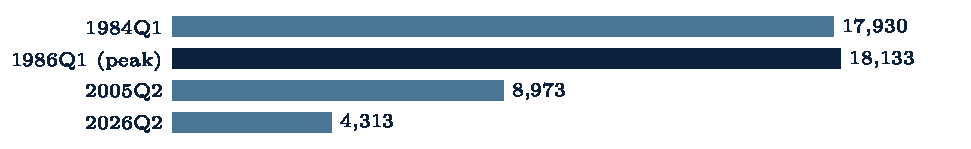
\includegraphics[width=.96\linewidth]{figures/archive_quarter_counts.pdf}\par
\captionof*{figure}{\textbf{Figure A1.} Reporting CERTs at selected quarters and at the archival maximum. Source: Phase 1, cell 47.}
\end{minipage}\par

\newpage

\section{Appendix B. Data Quality and Label
Audit}\label{appendix-b.-data-quality-and-label-audit}

\tabletag{B1}{Complete V2-to-V3 missing-label accounting}

\begin{longtable}[]{@{}lrrr@{}}
\toprule\noalign{}
V2 reason & V2 missing & Reclassified zero & V3 still missing \\
\midrule\noalign{}
\endhead
\bottomrule\noalign{}
\endlastfoot
Verified merger competing event & 55,754 & 55,754 & 0 \\
Event horizon right censored & 13,070 & 0 & 13,070 \\
Unresolved administrative exit & 7,514 & 7,514 & 0 \\
Financial-panel end & 4,273 & 4,273 & 0 \\
Verified competing closure & 1,714 & 1,714 & 0 \\
Unresolved missing endpoint & 1,646 & 1,646 & 0 \\
Pre-existing failure & 1,176 & 0 & 1,176 \\
Assistance & 504 & 504 & 0 \\
Quarantine & 70 & 0 & 70 \\
Partial continuation & 70 & 70 & 0 \\
\textbf{Total} & \textbf{85,791} & \textbf{71,475} & \textbf{14,316} \\
\end{longtable}

\notetext{Source: Phase 2 cells 412–418. No originally missing target became positive in this accounting.}

\textbf{Two observation clocks.} For 4,273 rows the financial panel ends
before continued reporting can be established. The registry still
provides a mature event window, so those rows can receive V3 zero. The
13,070 genuinely immature event windows keep their null label. I retain
a reason code for either case, and I retain the administrative review
flag on the 7,514 cases whose exit remains uncertain.

\textbf{Cohort sensitivity.} The Phase 5 split audit records
\textbf{4,371 fewer TRAIN rows}, \textbf{394 fewer Crisis rows} and
\textbf{2,097 fewer Recent OOT rows} under the strict V3 filter. These
are coverage counts. The archived scorecard uses the main cohort. The
development OOF comparison holds predictions and the fixed operating cut
constant and reapplies the strict filter by key. Table F4 reports the
fold-level result.

\textbf{Reconciliation.} The V3 rule resolves 83.3\% of the originally
missing V2 labels. The 14,316 labels still missing consist of 13,070
right-censored rows, 1,176 rows with pre-existing failure and 70
quarantined rows. Retaining these reason codes allows a replay to
distinguish newly mature event windows from origin-date exclusions and
source records requiring investigation.

When refreshing the event registry, I would tabulate transitions out of
each reason code alongside any change in the outcome cutoff. A later
cutoff can resolve a row with an immature horizon. Changes to a
quarantined record require separate evidence from the source registry.

\textbf{Institution linkage.} In the independent snapshot audit, 235
CERTs covering 10,996 bank-quarters lacked an institutions match. Five
matched CERTs covering 218 rows had a recorded end date before their
last financial report. These discrepancies identify cases for review
before using an administrative end date to define the eligible
population. The counts refer to linkage across the archival panel (Phase
2, cell 364).

\textbf{Composition of the recovered labels.} Verified mergers account
for 55,754 of the 71,475 resolved rows (78.0\%). Unresolved
administrative exits account for another 7,514 (10.5\%) and retain their
review flag. The two groups distinguish documented competing events from
zeros assigned under the administrative-exit policy.

\textbf{Eligibility in the archival panel.} Main V3 contains 1,668,293
eligible bank-quarters, including 10,852 positives. Strict V3 removes
7,514 flagged zeros (0.45\%), leaving 1,660,779 rows before W1 alignment
and temporal filtering (Phase 2, cells 409 and 414).

\chart{dated_failures}{Dated failures in Phase 2 by calendar year. The shaded band marks the 2008–2012 Crisis window. The recorded 2026 scope ends in Q2. Source: Phase 2 cell 201.}{.79}

\newpage

\subsection{B.2 Registry validation and boundary
tests}\label{b.2-registry-validation-and-boundary-tests}

\tabletag{B2}{Archived registry validation}

\begin{longtable}[]{@{}lr@{}}
\toprule\noalign{}
Measure & Records or CERTs \\
\midrule\noalign{}
\endhead
\bottomrule\noalign{}
\endlastfoot
Raw failure and assistance records & 4,117 \\
Quarantined for missing CERT & 488 \\
Quarantined for conflicting failure dates & 6 \\
Records after quarantine & 3,623 \\
Valid failure CERTs & 3,033 \\
Valid assistance events & 590 \\
\end{longtable}

\notetext{Source: Phase 2 cell 308. This registry is broader than the modelling windows. Records and unique CERTs have different units.}

\tabletag{B3}{Boundaries to verify in a label or vintage replay}

\begin{longtable}[]{@{}
  >{\raggedright\arraybackslash}p{(\columnwidth - 2\tabcolsep) * \real{0.5000}}
  >{\raggedright\arraybackslash}p{(\columnwidth - 2\tabcolsep) * \real{0.5000}}@{}}
\toprule\noalign{}
\begin{minipage}[b]{\linewidth}\raggedright
Case
\end{minipage} & \begin{minipage}[b]{\linewidth}\raggedright
Expected action and assertion
\end{minipage} \\
\midrule\noalign{}
\endhead
\bottomrule\noalign{}
\endlastfoot
Failure just before or on the origin & Exclude as pre-existing \\
Qualifying failure within the next four quarters & Positive with a
usable source date \\
Qualifying failure at fourth later quarter-end & Upper boundary is
inclusive \\
Qualifying failure after the fourth later quarter-end & Outside the
target \\
Verified merger with mature observation & Preserve competing-exit reason
and apply the V3 event rule \\
Event follow-up has not matured & Keep target unavailable under the
model eligibility rule \\
Historical report is revised after scoring & In a vintage replay use the
report version already available at scoring \\
Lag or report quarter is missing & Preserve the null where the formula
needs that exact quarter \\
\end{longtable}

\textbf{Denominator sensitivity.} Right censoring accounts for 13,070 of
the 14,316 labels still missing under V3, or 91.3\%. V3 assigns zero to
the 7,514 unresolved administrative exits and retains a flag for cohort
sensitivity. A strict-cohort rerun would keep the fitted scorer and
review policy fixed, and report the change in eligible banks, positive
banks and detected banks. The positive-bank count is the recall
denominator. The eligible-bank count shows the size of the screened
population.

Phase 2 validates the input key independently before joining the event
registry and matches the institution reference separately. I count
unmatched and ambiguous cases and compare output keys with the input. I
also verify that the fit allowlist contains none of the event-history or
disposition fields. These checks prevent an accidental many-to-many
merge or future outcome columns from affecting the number or content of
predictor rows.

The final as-of question needs a second artifact: receipt and revision
metadata for each source report. With that artifact, I would compare the
earliest permissible first alert against the verified failure date and
record the scoring timestamp. After a rule change I would repeat the
same boundary tests and record any affected bank--quarters by reason
code.

For a validation Top 25 replay, compare detections among banks eligible
in both cohorts. Removing flagged rows can free review slots. The common
bank set helps separate that queue effect from a change in bank support.

\textbf{Field sparsity and capital transitions.} The historical scan
flagged 79,921 rows across 4,086 banks with more than half of the
audited financial fields missing. In the negative-equity transition
audit, 908 observations lacked an observable onset and 26 had a large
contemporaneous asset change flagged for accounting or restructuring
review. The diagnostics record whether the history supports a transition
classification and preserve the underlying rows for later analysis
(Phase 2, cell 370).

\par\addvspace{5pt}\noindent
\begin{minipage}{\linewidth}\centering
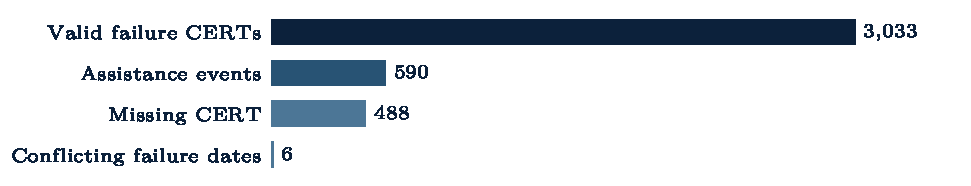
\includegraphics[width=.90\linewidth]{figures/registry_validation_counts.pdf}\par
\captionof*{figure}{\textbf{Figure B1.} Registry validation counts. Quarantine: 494 of 4,117 records (12.0\%). Phase 2, cell 308.}
\end{minipage}\par

\newpage

\section{Appendix C. Processing Benchmarks and Spark
Parity}\label{appendix-c.-processing-benchmarks-and-spark-parity}

\subsection{C.1 Comparison harness and plan
evidence}\label{c.1-comparison-harness-and-plan-evidence}

The one-to-one parity join checks keys, null masks, nonfinite values and
numeric deviations. For finite values the tolerance is
\(10^{-8}+10^{-6}|x_{\mathrm{ref}}|\) against the right-hand series.

\tabletag{C1}{Observed plans and scope of feature-equivalence tests}

\begin{longtable}[]{@{}
  >{\raggedright\arraybackslash}p{(\columnwidth - 4\tabcolsep) * \real{0.3333}}
  >{\raggedright\arraybackslash}p{(\columnwidth - 4\tabcolsep) * \real{0.3333}}
  >{\raggedright\arraybackslash}p{(\columnwidth - 4\tabcolsep) * \real{0.3333}}@{}}
\toprule\noalign{}
\begin{minipage}[b]{\linewidth}\raggedright
Evidence
\end{minipage} & \begin{minipage}[b]{\linewidth}\raggedright
What I checked
\end{minipage} & \begin{minipage}[b]{\linewidth}\raggedright
Archived result
\end{minipage} \\
\midrule\noalign{}
\endhead
\bottomrule\noalign{}
\endlastfoot
Polars optimized scan & Read projection and date range before fixed
window & 11 of 141 columns projected \\
Polars output boundary & 2024 filter remains distinct from source
lookback & Prior 2023 observations retained \\
Spark vs pandas and Polars, 2024 & Key-by-key check of all nine features
& Zero failing comparisons \\
pandas to Polars historical & Blocks across the full archive with
one-year lookback & Independent historical parity checks \\
Spark physical plan & Sort-merge joins, exchanges and final sort & Four
joins, six exchanges \\
\end{longtable}

\notetext{Source: Phase 3 §§3.5, 3.6.4 and 3.9.2. Spark W1 uses 2024 with 2023 lookback.}

\textbf{Scale by bank history.} With intact bank histories, input grew
from 422,267 to 1,682,616 rows (3.98-fold) and median runtime from 0.359
to 1.173 seconds (3.27-fold). At 50\%, 837,797 rows took 0.506 seconds.

\tabletag{C2}{Phase 3 layout A/B on matched 1993–2024 input}

\begin{longtable}[]{@{}
  >{\raggedright\arraybackslash}p{(\columnwidth - 8\tabcolsep) * \real{0.2000}}
  >{\raggedleft\arraybackslash}p{(\columnwidth - 8\tabcolsep) * \real{0.2000}}
  >{\raggedleft\arraybackslash}p{(\columnwidth - 8\tabcolsep) * \real{0.2000}}
  >{\raggedleft\arraybackslash}p{(\columnwidth - 8\tabcolsep) * \real{0.2000}}
  >{\raggedleft\arraybackslash}p{(\columnwidth - 8\tabcolsep) * \real{0.2000}}@{}}
\toprule\noalign{}
\begin{minipage}[b]{\linewidth}\raggedright
Layout
\end{minipage} & \begin{minipage}[b]{\linewidth}\raggedleft
Size (MiB)
\end{minipage} & \begin{minipage}[b]{\linewidth}\raggedleft
Full scan (ms)
\end{minipage} & \begin{minipage}[b]{\linewidth}\raggedleft
2024 scan (ms)
\end{minipage} & \begin{minipage}[b]{\linewidth}\raggedleft
Candidate groups for 2024
\end{minipage} \\
\midrule\noalign{}
\endhead
\bottomrule\noalign{}
\endlastfoot
Snappy, 50k rows/group & 334.39 & 61.29 & 7.58 & 2 / 22 \\
ZSTD, 50k rows/group & 238.10 & 69.89 & 10.35 & 2 / 22 \\
ZSTD, 10k rows/group & 244.75 & 89.48 & 15.62 & 3 / 106 \\
ZSTD, annual & 239.56 & 77.06 & 27.87 & 1 / 34 \\
\end{longtable}

\notetext{Source: Phase 3 §§3.8.3–3.8.4, 24 timed scans. Candidate groups are metadata estimates.}

ZSTD 50k saves 28.79\% of disk space and takes 8.60 ms longer on the
full scan than Snappy 50k. Smaller ZSTD row groups increase potential
pruning and take longer on the observed selective scan.

\textbf{Spark batch architecture.} The Phase 3 §3.9.6 Wide comparison
checks 133 fields and six statistics per field. Median elapsed time was
\textbf{5.390 s} for direct batch scans and \textbf{5.598 s} for cached
batches, including 0.412 s to materialize the cache. Both strategies
passed numerical parity. Each has two repetitions, so the small observed
gap warrants caution.

\textbf{Low-memory output and cluster verification.} Phase 3 §3.6.4a
wrote 103 batches in 49.70 s via a driver-side partition iterator and
verified 1,682,616 keys and 20 columns. A matched cluster run could
measure throughput, I/O, shuffle, spill and executor RAM.

\textbf{Full-archive codec check.} The full-source experiment covers
1,682,616 rows, distinct from the matched 1993-2024 layout test in Table
C2. Both 50k-row-group layouts passed value-fidelity checks in all 43
calendar years. ZSTD used 354.94 MiB versus 498.23 MiB for Snappy, a
28.76\% reduction. Median full scans were 62.59 and 63.15 ms,
respectively (Phase 3, cell 97).

\textbf{Repeated Spark actions.} The local cache test reduced the median
repeated action from 339.90 to 314.52 ms across three runs, with a
separate 1,178.1 ms setup cost. At those medians and assuming equal
savings across repeated actions, the setup would break even after about
47 actions on the same workload (Phase 3, cell 117).

\textbf{Controlled 2024 scan of W1 inputs.} Phase 3 held 18,399 rows and
the same 11 raw input columns fixed. The resulting CSV occupied 4.049
MiB and ZSTD Parquet 0.613 MiB, an 84.9\% reduction. Across five
warm-cache timings, the median scan fell from 9.685 to 6.335 ms. The
observed ranges were 8.379-10.498 ms for CSV and 3.581-6.846 ms for
Parquet. The benchmark verified the values before timing.

The test measures reading and materializing the selected columns. A
production W1 request also needs historical lookback and feature
calculation. This distinction explains why the narrow A/B timings are
reported alongside the full-source layout and matched engine results
(Phase 3, cells 101-102).

\newpage

\section{Appendix D. Feature Dictionary and
Interpretation}\label{appendix-d.-feature-dictionary-and-interpretation}

\tabletag{D1}{Complete nine-variable W1 dictionary}

\begin{longtable}[]{@{}
  >{\raggedright\arraybackslash}p{(\columnwidth - 2\tabcolsep) * \real{0.5000}}
  >{\raggedright\arraybackslash}p{(\columnwidth - 2\tabcolsep) * \real{0.5000}}@{}}
\toprule\noalign{}
\begin{minipage}[b]{\linewidth}\raggedright
W1 feature
\end{minipage} & \begin{minipage}[b]{\linewidth}\raggedright
Formula or observation requirement
\end{minipage} \\
\midrule\noalign{}
\endhead
\bottomrule\noalign{}
\endlastfoot
\texttt{equity\_to\_assets} & EQ / ASSET \\
\texttt{deposits\_to\_assets} & DEP / ASSET \\
\texttt{cash\_to\_assets} & CHBAL / ASSET \\
\texttt{securities\_to\_assets} & SC / ASSET \\
\texttt{core\_deposit\_share} & COREDEP / DEP \\
\texttt{noncurrent\_loan\_ratio} & NCLNLS / LNLSGR \\
\texttt{asset\_growth\_4q} & ASSET at the origin / ASSET exactly four
quarters earlier − 1 \\
\texttt{roa\_rolling\_mean\_4q} & Mean of four finite, exact quarterly
ROA values \\
\texttt{roa\_rolling\_std\_4q} & Sample deviation of the same four
values \\
\end{longtable}

\notetext{Source: Phase 3 §3.4. Use current or historical reports available by scoring time. Current ratios require finite numerators and positive finite denominators. W1 is keyed by reporting quarter. Actual release vintages remain incomplete.}

\tabletag{D2}{Recency-weighted RF split importance (MDI)}

\begin{longtable}[]{@{}
  >{\raggedright\arraybackslash}p{(\columnwidth - 6\tabcolsep) * \real{0.2500}}
  >{\raggedleft\arraybackslash}p{(\columnwidth - 6\tabcolsep) * \real{0.2500}}
  >{\raggedright\arraybackslash}p{(\columnwidth - 6\tabcolsep) * \real{0.2500}}
  >{\raggedleft\arraybackslash}p{(\columnwidth - 6\tabcolsep) * \real{0.2500}}@{}}
\toprule\noalign{}
\begin{minipage}[b]{\linewidth}\raggedright
RF feature
\end{minipage} & \begin{minipage}[b]{\linewidth}\raggedleft
Share
\end{minipage} & \begin{minipage}[b]{\linewidth}\raggedright
RF feature
\end{minipage} & \begin{minipage}[b]{\linewidth}\raggedleft
Share
\end{minipage} \\
\midrule\noalign{}
\endhead
\bottomrule\noalign{}
\endlastfoot
RBC1AAJ & 0.13651 & ROA & 0.05646 \\
RBCRWAJ & 0.11204 & ROA, 4Q mean & 0.03647 \\
Equity/assets & 0.10086 & ROA, 4Q deviation & 0.02519 \\
Noncurrent loan share & 0.08419 & ROE & 0.02511 \\
Noncurrent loans × earnings & 0.06810 & Equity (EQ) & 0.02009 \\
Expense burden × earnings & 0.06718 & ORE & 0.01842 \\
Equity/assets squared & 0.06497 & Asset growth × noncurrent share &
0.01700 \\
& & Net charge-off, 4Q volatility & 0.01190 \\
\end{longtable}

\notetext{Source: nháp\_v2 §5.5A-RF. MDI is a summary of tree splits in the frozen challenger.}

\textbf{Reading the capital measures together.} The three leading
capital measures account for 34.94\% of impurity-based importance.
Regulatory capital ratios and book equity can carry overlapping
information. A grouped permutation on held-out development data could
test their joint contribution to ranking. I would permute the inputs
together, keeping equity/assets and its squared term aligned, and
rescore each fold with its fitted model. I would report changes in AP
and bank recall at the original quarterly budget.

The squared equity/assets term carries another 6.50\% of split
importance. Its inclusion shows that the fitted trees split on two
representations of the same underlying ratio. I would report permutation
results by fold to see whether the combined contribution is stable
across reporting periods.

\textbf{Ordered inventories.} The LightGBM feature inventory is
reproduced separately in the source archive. For the RF challenger, the
release specification records the fitted feature order. Interest,
expense and deposit fields require reporting-regime checks before
domestic use. In the separate Phase 4 stability audit, three Top-40
lists shared 33 fields and had a union of 48.

\textbf{Annual coverage and interpretation.} In an exploratory
availability audit of 102 candidate fields over 1985-2006, 50 reached
95\% coverage every year, 26 had broad coverage, 15 had moderate
instability and 11 depended on the reporting regime. For example, RBCT2
was completely missing in its worst year, and more than 60\% of values
were missing in five years. Phase 4, cell 27, records availability
patterns for reviewing inputs separately from the model feature
inventories and split-importance table.

\textbf{Cross-group redundancy.} All 17 cross-group pairs above the 0.98
absolute-correlation threshold were classified as high correlation only.
For example, substituting total risk-based capital for book equity would
change coverage on 62,624 rows with mismatched missingness flags (Phase
4, cell 72).

\textbf{Deposit growth checks.} In the extreme-growth audit, 14 cases
had prior-year deposits from 1 to 53 in source units, and nine had
balances from 27,886 to 57,000. Review both small denominators and large
reported balance changes (Phase 4, cell 126).

\newpage

\section{Appendix E. Validation Design and Alarm
Policy}\label{appendix-e.-validation-design-and-alarm-policy}

\tabletag{E1}{Chronological fold schedule and recency-weighted RF validation}

\begin{longtable}[]{@{}
  >{\raggedright\arraybackslash}p{(\columnwidth - 12\tabcolsep) * \real{0.0769}}
  >{\raggedright\arraybackslash}p{(\columnwidth - 12\tabcolsep) * \real{0.1692}}
  >{\raggedleft\arraybackslash}p{(\columnwidth - 12\tabcolsep) * \real{0.1077}}
  >{\raggedright\arraybackslash}p{(\columnwidth - 12\tabcolsep) * \real{0.1846}}
  >{\raggedleft\arraybackslash}p{(\columnwidth - 12\tabcolsep) * \real{0.1538}}
  >{\raggedleft\arraybackslash}p{(\columnwidth - 12\tabcolsep) * \real{0.1385}}
  >{\raggedleft\arraybackslash}p{(\columnwidth - 12\tabcolsep) * \real{0.1692}}@{}}
\toprule\noalign{}
\begin{minipage}[b]{\linewidth}\raggedright
Fold
\end{minipage} & \begin{minipage}[b]{\linewidth}\raggedright
Fit years
\end{minipage} & \begin{minipage}[b]{\linewidth}\raggedleft
Purge
\end{minipage} & \begin{minipage}[b]{\linewidth}\raggedright
Validation
\end{minipage} & \begin{minipage}[b]{\linewidth}\raggedleft
Positive banks
\end{minipage} & \begin{minipage}[b]{\linewidth}\raggedleft
RF AP
\end{minipage} & \begin{minipage}[b]{\linewidth}\raggedleft
Bank recall@25
\end{minipage} \\
\midrule\noalign{}
\endhead
\bottomrule\noalign{}
\endlastfoot
F1 & 1985--1986 & 1987 & 1988--1990 & 1,347 & 0.47321 & 12.32\% \\
F2 & 1985--1990 & 1991 & 1992--1994 & 194 & 0.34576 & 38.14\% \\
F3 & 1985--1995 & 1996 & 1997--2000 & 23 & 0.14323 & 65.22\% \\
F4 & 1985--2000 & 2001 & 2002--2004 & 12 & 0.08263 & 58.33\% \\
\end{longtable}

\tabletag{E2}{Recency-weighted RF threshold grid for development cost minimization}

\begin{longtable}[]{@{}rrrrrr@{}}
\toprule\noalign{}
Cut & F1--F3 hits & Misses & False alerts & F4 hits & F4 false alerts \\
\midrule\noalign{}
\endhead
\bottomrule\noalign{}
\endlastfoot
0.13434 & 1,465 & 99 & 18,098 & 7 & 691 \\
0.13832 & 1,462 & 102 & 17,611 & 7 & 667 \\
0.17272 & 1,436 & 128 & 14,151 & 7 & 522 \\
0.19191 & 1,416 & 148 & 12,701 & 7 & 466 \\
0.21110 & 1,398 & 166 & 11,498 & 7 & 404 \\
0.23989 & 1,374 & 190 & 9,991 & 7 & 337 \\
No alert & 0 & 1,564 & 0 & 0 & 0 \\
\end{longtable}

\notetext{Source: nháp\_v2 §5.3B-SENS. Hits count positive bank–folds in F1–F3 and positive banks in F4. Displayed cuts are rounded.}

The F3 cut minimizes this recorded grid only at avoidable-loss shares of
about 0.303\%--0.329\%. The limits come from ties with 0.21110 and
0.17272. This interval is a retrospective sensitivity result.

\tabletag{E3}{Review allocation on recency-weighted validation OOF scores}

\begin{longtable}[]{@{}
  >{\raggedright\arraybackslash}p{(\columnwidth - 8\tabcolsep) * \real{0.2000}}
  >{\raggedleft\arraybackslash}p{(\columnwidth - 8\tabcolsep) * \real{0.2000}}
  >{\raggedleft\arraybackslash}p{(\columnwidth - 8\tabcolsep) * \real{0.2000}}
  >{\raggedleft\arraybackslash}p{(\columnwidth - 8\tabcolsep) * \real{0.2000}}
  >{\raggedleft\arraybackslash}p{(\columnwidth - 8\tabcolsep) * \real{0.2000}}@{}}
\toprule\noalign{}
\begin{minipage}[b]{\linewidth}\raggedright
Review policy
\end{minipage} & \begin{minipage}[b]{\linewidth}\raggedleft
Hits / 1,576
\end{minipage} & \begin{minipage}[b]{\linewidth}\raggedleft
False alerts
\end{minipage} & \begin{minipage}[b]{\linewidth}\raggedleft
Repeat share
\end{minipage} & \begin{minipage}[b]{\linewidth}\raggedleft
Earlier hits
\end{minipage} \\
\midrule\noalign{}
\endhead
\bottomrule\noalign{}
\endlastfoot
Top 25 & 262 & 912 & 49.54\% & 0 \\
22 + 3 & 262 & 912 & 46.00\% & 3 \\
20 + 5 & 266 & 911 & 43.38\% & 5 \\
\end{longtable}

\textbf{Trade-offs by fold.} The 20+5 policy detects five bank--folds
missed by Top 25 and loses one previously detected bank--fold, for a net
gain of four under the same 1,300-review budget. F4 loses one detection
under 20+5 and contains only 12 positive banks. One bank therefore
changes F4 recall by 8.33 percentage points. Reporting the fold counts
alongside the pooled gain makes this trade-off visible.

\tabletag{E4}{Institutional coverage under the same quarterly review budget}

\begin{longtable}[]{@{}
  >{\raggedright\arraybackslash}p{(\columnwidth - 10\tabcolsep) * \real{0.1667}}
  >{\raggedleft\arraybackslash}p{(\columnwidth - 10\tabcolsep) * \real{0.1667}}
  >{\raggedleft\arraybackslash}p{(\columnwidth - 10\tabcolsep) * \real{0.1667}}
  >{\raggedleft\arraybackslash}p{(\columnwidth - 10\tabcolsep) * \real{0.1667}}
  >{\raggedleft\arraybackslash}p{(\columnwidth - 10\tabcolsep) * \real{0.1667}}
  >{\raggedleft\arraybackslash}p{(\columnwidth - 10\tabcolsep) * \real{0.1667}}@{}}
\toprule\noalign{}
\begin{minipage}[b]{\linewidth}\raggedright
Fold
\end{minipage} & \begin{minipage}[b]{\linewidth}\raggedleft
Positive banks
\end{minipage} & \begin{minipage}[b]{\linewidth}\raggedleft
Top 25 hits
\end{minipage} & \begin{minipage}[b]{\linewidth}\raggedleft
20 + 5 hits
\end{minipage} & \begin{minipage}[b]{\linewidth}\raggedleft
Change in hits
\end{minipage} & \begin{minipage}[b]{\linewidth}\raggedleft
Change in false alerts
\end{minipage} \\
\midrule\noalign{}
\endhead
\bottomrule\noalign{}
\endlastfoot
F1 & 1,347 & 166 & 167 & +1 & +1 \\
F2 & 194 & 74 & 78 & +4 & −3 \\
F3 & 23 & 15 & 15 & 0 & 0 \\
F4 & 12 & 7 & 6 & −1 & +1 \\
\end{longtable}

\notetext{Source: nháp\_v2, review-allocation experiment. Changes are 20 + 5 minus Top 25. Pooled bank recall rises from 16.62\% to 16.88\%.}

\tabletag{E5}{Best positive-quarter rank per bank on development OOF scores}

\begin{longtable}[]{@{}lrrrr@{}}
\toprule\noalign{}
Fold & Ranks 1-25 & Ranks 26-35 & Ranks 36-50 & Ranks above 50 \\
\midrule\noalign{}
\endhead
\bottomrule\noalign{}
\endlastfoot
F1 & 166 & 44 & 67 & 1,070 \\
F2 & 74 & 19 & 17 & 84 \\
F3 & 15 & 0 & 1 & 7 \\
F4 & 7 & 0 & 0 & 5 \\
\end{longtable}

Each positive bank enters one bin per fold. Ranks 26-50 include 111
banks in F1 and 36 in F2. All five F4 misses at Top 25 also miss Top 50
(Phase 5, cell 316).

\newpage

\section{Appendix F. Test Diagnostics and
Robustness}\label{appendix-f.-test-diagnostics-and-robustness}

\subsection{F.1 Precision--recall and review
capacity}\label{f.1-precisionrecall-and-review-capacity}

\chart{current_rf_pr}{Recency-weighted RF precision–recall by bank–quarter. Curves and AP come from the matching notebook run. Source: nháp\_v2 §§5.4B and 5.4B-PLOT.}{.79}

\tabletag{F1}{Recency-weighted RF capacity ladder}

\begin{longtable}[]{@{}
  >{\raggedright\arraybackslash}p{(\columnwidth - 10\tabcolsep) * \real{0.1667}}
  >{\raggedleft\arraybackslash}p{(\columnwidth - 10\tabcolsep) * \real{0.1667}}
  >{\raggedleft\arraybackslash}p{(\columnwidth - 10\tabcolsep) * \real{0.1667}}
  >{\raggedleft\arraybackslash}p{(\columnwidth - 10\tabcolsep) * \real{0.1667}}
  >{\raggedleft\arraybackslash}p{(\columnwidth - 10\tabcolsep) * \real{0.1667}}
  >{\raggedleft\arraybackslash}p{(\columnwidth - 10\tabcolsep) * \real{0.1667}}@{}}
\toprule\noalign{}
\begin{minipage}[b]{\linewidth}\raggedright
Window
\end{minipage} & \begin{minipage}[b]{\linewidth}\raggedleft
K per quarter
\end{minipage} & \begin{minipage}[b]{\linewidth}\raggedleft
Total reviews
\end{minipage} & \begin{minipage}[b]{\linewidth}\raggedleft
Correct reviews
\end{minipage} & \begin{minipage}[b]{\linewidth}\raggedleft
False alerts
\end{minipage} & \begin{minipage}[b]{\linewidth}\raggedleft
Banks hit
\end{minipage} \\
\midrule\noalign{}
\endhead
\bottomrule\noalign{}
\endlastfoot
Crisis & 10 & 200 & 175 & 25 & 144/487 \\
Crisis & 25 & 500 & 408 & 92 & 278/487 \\
Crisis & 35 & 700 & 548 & 152 & 330/487 \\
Crisis & 50 & 1,000 & 717 & 283 & 377/487 \\
Recent OOT & 10 & 460 & 88 & 372 & 38/53 \\
Recent OOT & 25 & 1,150 & 119 & 1,031 & 44/53 \\
Recent OOT & 35 & 1,610 & 126 & 1,484 & 44/53 \\
Recent OOT & 50 & 2,300 & 134 & 2,166 & 44/53 \\
\end{longtable}

\chart{review_capacity}{Detection and false reviews as the quarterly budget changes. Source: nháp\_v2 §5.4B-PLOT.}{.79}

Correct reviews count alerts on positive bank--quarters. Banks hit
counts each institution once if an alert falls inside any of its
positive quarters.

\textbf{Marginal review burden.} In Crisis, moving from Top 25 to Top 35
required about 1.15 additional false alerts per extra bank detected
(60/52). The move from Top 35 to Top 50 required 2.79 (131/47). In
Recent OOT, the two expansions added 453 and 682 false alerts,
respectively, with 44 of 53 banks detected at all three budgets. They
produced seven and eight more correct bank--quarter reviews,
respectively. Row-level gains can therefore coexist with unchanged
institutional coverage.

\textbf{Timing at equal bank coverage.} In Recent OOT, both policies
first flagged 34 banks in the same quarter and missed nine. The fixed
cutoff led for nine banks, including two by three quarters, and Top 25
led for one bank by two quarters. The additional 594 false alerts at the
fixed cutoff buy earlier review for some banks already covered (Phase 5,
cell 373).

\newpage

\fontsize{10pt}{11.75pt}\selectfont

\subsection{F.2 Annual rankings, uncertainty and
calibration}\label{f.2-annual-rankings-uncertainty-and-calibration}

\tabletag{F2}{Recency-weighted RF annual AP and positive-quarter support}

\begin{longtable}[]{@{}rrrrrr@{}}
\toprule\noalign{}
Crisis year & Positives & AP & Recent year & Positives & AP \\
\midrule\noalign{}
\endhead
\bottomrule\noalign{}
\endlastfoot
2008 & 355 & 0.46240 & 2014 & 46 & 0.55005 \\
2009 & 670 & 0.72157 & 2015 & 23 & 0.34909 \\
2010 & 457 & 0.75994 & 2016 & 29 & 0.64555 \\
2011 & 269 & 0.71358 & 2017 & 9 & 0.41176 \\
2012 & 129 & 0.70508 & 2018 & 6 & 0.04102 \\
& & & 2019 & 19 & 0.44017 \\
& & & 2020 & 7 & 0.75763 \\
& & & 2021 & 0 & --- \\
& & & 2022 & 14 & 0.00116 \\
& & & 2023 & 9 & 0.15398 \\
& & & 2024 & 9 & 0.00308 \\
& & & 2025 through Q2 & 4 & 0.48275 \\
\end{longtable}

\tabletag{F3}{External CERT-clustered bootstrap intervals}

\begin{longtable}[]{@{}lrr@{}}
\toprule\noalign{}
Window and scorer & AP interval & Bank recall at Top 1\% \\
\midrule\noalign{}
\endhead
\bottomrule\noalign{}
\endlastfoot
Crisis, LightGBM & 0.610--0.675 & 81.29--88.78\% \\
Crisis, recency-weighted RF & 0.600--0.669 & 83.43--89.01\% \\
Recent OOT, LightGBM & 0.229--0.417 & 71.79--92.70\% \\
Recent OOT, recency-weighted RF & 0.275--0.474 & 71.79--92.70\% \\
\end{longtable}

\notetext{Sources: nháp\_v2 cells 347 and 351. The external bootstrap uses 150 draws by CERT. Top 1\% differs from Top 25 per quarter. AP is undefined when a year has no positives.}

\chartpair{annual_ap}{calibration_skill}{Left: annual AP. Right: Brier skill relative to the observed-prevalence baseline. Sources: nháp\_v2 cells 347 and 371.}

RF Brier improves from 0.014240 to 0.007335 in Crisis and from 0.002080
to 0.000786 in Recent after isotonic calibration. Calibrated Brier skill
is 37.67\% in Crisis and −12.18\% in Recent. I retain raw scores for
ranking because calibration creates ties. The optional strict-cohort
refit remains disabled. The Strict V3 development comparison uses the
existing scores.

\tabletag{F4}{Development OOF exclusion and information-delay sensitivity}

\begin{longtable}[]{@{}
  >{\raggedright\arraybackslash}p{(\columnwidth - 8\tabcolsep) * \real{0.2000}}
  >{\raggedleft\arraybackslash}p{(\columnwidth - 8\tabcolsep) * \real{0.2000}}
  >{\raggedleft\arraybackslash}p{(\columnwidth - 8\tabcolsep) * \real{0.2000}}
  >{\raggedleft\arraybackslash}p{(\columnwidth - 8\tabcolsep) * \real{0.2000}}
  >{\raggedleft\arraybackslash}p{(\columnwidth - 8\tabcolsep) * \real{0.2000}}@{}}
\toprule\noalign{}
\begin{minipage}[b]{\linewidth}\raggedright
Fold
\end{minipage} & \begin{minipage}[b]{\linewidth}\raggedleft
Strict rows excluded
\end{minipage} & \begin{minipage}[b]{\linewidth}\raggedleft
Main / Strict AP
\end{minipage} & \begin{minipage}[b]{\linewidth}\raggedleft
Prior-score match
\end{minipage} & \begin{minipage}[b]{\linewidth}\raggedleft
AP change, prior vs current
\end{minipage} \\
\midrule\noalign{}
\endhead
\bottomrule\noalign{}
\endlastfoot
F1 & 1,582 & 0.47321 / 0.49920 & 90.64\% & −13.80\% \\
F2 & 529 & 0.34576 / 0.41935 & 90.97\% & −35.71\% \\
F3 & 73 & 0.14323 / 0.14338 & 92.72\% & −52.71\% \\
F4 & 87 & 0.08263 / 0.08540 & 91.12\% & −63.59\% \\
\end{longtable}

The strict filter excludes zero positive bank--quarters. Match shares
refer to the original OOF rows in each fold. The current- and
prior-score AP comparison uses the same matched rows in each fold.

\textbf{Calibration transfer within development.} Against historical
prevalence, unweighted isotonic led in F2 (Brier skill of +5.57\% vs
+5.14\% for recency-weighted isotonic). The weighted method led in F3
(+21.36\% vs +18.02\%). All six methods had negative skill against the
prevalence observed in F4. The fold results show how the comparison
depends on both the validation period and the prevalence benchmark
(Phase 5, cell 339).

\newpage

\fontsize{10pt}{11.75pt}\selectfont

\section{Appendix G. Reproduction
Checklist}\label{appendix-g.-reproduction-checklist}

\tabletag{G1}{Artifacts and evidence required for a clean rerun}

\begin{longtable}[]{@{}
  >{\raggedright\arraybackslash}p{(\columnwidth - 4\tabcolsep) * \real{0.3333}}
  >{\raggedright\arraybackslash}p{(\columnwidth - 4\tabcolsep) * \real{0.3333}}
  >{\raggedright\arraybackslash}p{(\columnwidth - 4\tabcolsep) * \real{0.3333}}@{}}
\toprule\noalign{}
\begin{minipage}[b]{\linewidth}\raggedright
Step
\end{minipage} & \begin{minipage}[b]{\linewidth}\raggedright
Source/output to locate
\end{minipage} & \begin{minipage}[b]{\linewidth}\raggedright
Verify before release
\end{minipage} \\
\midrule\noalign{}
\endhead
\bottomrule\noalign{}
\endlastfoot
Environment & README, pinned requirements, Git commit & Python, Java,
Spark, Polars, PyArrow, CPU/RAM and seeds \\
Phases 0--1 & Field contract, Raw manifests, annual Bronze & 170
quarters, expected reference totals, keys and Raw--Bronze
reconciliation \\
Phases 2--3 & Silver, V3 handoff and W1 & 20 quality gates, versioned
outcome logic, 1,610,856 W1 keys and matched features for parity \\
Phase 4 & Gold Parquet and Phase 4→5 export JSON, Top 40 metadata &
REPDTE maximum, eligible populations, ordered predictors and digests \\
Phase 5 development & OOF, selected estimator, calibrator, freeze spec &
Fold boundaries, seed 4903, preselected metrics and policy, prediction
read-back \\
Phase 5 external & Access log, scorecard and keyed predictions & Match
checksums, confirm role of prior accesses, assert cutoff, preserve score
outputs \\
\end{longtable}

\textbf{Notebook anchors.} The Phase 2 handoff records labels, source
audits and age policies. In Phase 4--5, the split (index 298), RF
strategies and bootstrap (308--314) and initial calibration/cut
(325--327) retain their positions. Development sensitivities appear at
330, 333, 336 and 339. The original refit and external sequence
(331--334 in the archived source) is now at 343--346. Original test
diagnostics (335--339, 343) are now at 347--351, 355. Validation review
allocation moved from 360 to 376.

\textbf{Freeze and access evidence.} The refit output records the
release created on 25 November 2026. Its specification SHA-256 is
printed below. The run's verifier matches the spec and model components
before scoring. It writes \texttt{external\_test\_access.json} with a
first-access UTC timestamp and the bound digests. An existing log is
accepted only when the recorded release digests match. The archived
scoring cell shows one pass for the submitted evaluation.

\begin{verbatim}
be8f1b5c5c2a7bf5883ae38bcaf22b4706805425c32fa7e963b7880dfba6314c
\end{verbatim}

\textbf{Point-in-time evidence.} Phase 2 cell 374 records zero matched,
verified bank--quarter release timestamps. Cell 387 exports a
conservative proxy and delay scenarios. For a production replay, pin an
actual release-date source and join by CERT and REPDTE before scoring.
Preserve the as-published vintage, filing corrections and the decision
timestamp.

\textbf{Reproduction status.} The report builds from source, and the
discrete cost grid has an independent check. The read-only audit records
artifact and schema integrity alongside archived notebook outputs. A
full replay requires matching local FDIC snapshots and handoffs. An API
refresh creates a release with separate digests.

\textbf{Audited Python 3.13.7 dependencies.} pandas 2.3.3, NumPy 2.3.3,
Polars 2.1.0, scikit-learn 1.9.0, LightGBM 4.7.0, PyArrow 26.0.1, joblib
1.5.2, SciPy 1.16.3, Matplotlib 3.10.7, psutil 7.0.0 and PySpark 4.1.4.

\textbf{Audit coverage.} The six pinned file-digest checks covered the
Phase 2 V3 labels, the Phase 4 LightGBM model and model metadata, the
Phase 5 recency-weighted forest and both calibrators. Presence checks
covered the Phase 0 field handoff, data scope and bundle manifest, the
financial schema and the frozen-specification file. The specification
passed a separate internal digest check. Gold was audited for schema and
required-field presence (Phase 5, cell 362).

\textbf{Scoring and drift checks.} The scoring function expects
engineered inputs and takes the latest eligible report per CERT under a
45- or 90-day release-delay scenario. It returns the raw ranking,
calibrated probability and separate fixed-cutoff alert. The drift check
holds training quantile bins fixed and includes missing values in their
own bin. The supplied synthetic check verifies that identical inputs
produce negligible PSI (Phase 5, cells 365-366).

\clearpage

\fontsize{11.8pt}{14.32pt}\selectfont
\setlength{\parskip}{5pt plus .8pt minus .3pt}
\renewcommand{\arraystretch}{1.16}
\renewcommand{\parttag}{References}

\section{References}\label{references}

Phase 0 uses exactly the 26 sources R01--R26. Historical design
references {[}H{]} and other sources follow. AI-use disclosure
{[}9{]}.\footnote{\fontsize{8.5bp}{10.2bp}\selectfont OpenAI ChatGPT and Codex (2026) were used to assist with code development, debugging, methodological discussions, experimental design, result interpretation, report editing, and documentation. Empirical results were obtained from the executed research notebooks. The author remains responsible for the methodology, verification of results, and final submitted content.}

\begin{multicols}{2}
\fontsize{8.5bp}{9.35bp}\selectfont
\setlength{\parskip}{1.15pt}
\raggedright
\reflisting{R01}{Ekinci and Sen (2024). \href{https://link.springer.com/article/10.1007/s10614-023-10537-6}{Forecasting Bank Failure in the U.S.: A Cost-Sensitive Approach}.}
\reflisting{R02}{Alzayed, Eskandari and Yazdifar (2023). \href{https://link.springer.com/article/10.1007/s11156-023-01158-z}{Bank failure prediction: corporate governance and financial indicators}.}
\reflisting{R03}{Gunonu, Altun and Cavus (2026). \href{https://link.springer.com/article/10.1007/s10614-026-11353-4}{Explainable Bank Failure Prediction Models: Counterfactual Explanations to Reduce the Failure Risk}.}
\reflisting{R04}{Jev et al. (2026). \href{https://www.open-access.bcu.ac.uk/17298}{A systematic literature review of bank failure prediction models}.}
\reflisting{R05}{Citterio (2024). \href{https://www.sciencedirect.com/science/article/pii/S003801212400017X}{Bank failure prediction models: Review and outlook}.}
\reflisting{R06}{Bhat, Hanna and Shaw (2024). \href{https://scholar.smu.edu/business_accounting_research/147}{Why Do Some Troubled Banks Fail Instead of Merge?}.}
\reflisting{R07}{Oshinsky and Olin (2005). \href{https://archive.fdic.gov/view/fdic/12047}{Troubled Banks: Why Don't They All Fail?}.}
\reflisting{R08}{Beretta, Heuchenne and Restaino (2022). \href{https://pmc.ncbi.nlm.nih.gov/articles/PMC9639486}{Competing risks proportional-hazards cure model and generalized extreme value regression: an application to bank failures and acquisitions in the United States}.}
\reflisting{R09}{Li, Feng and Tang (2022). \href{https://pmc.ncbi.nlm.nih.gov/articles/PMC8928719}{Bank efficiency and failure prediction: a nonparametric and dynamic model based on data envelopment analysis}.}
\reflisting{R10}{Suss and Treitel (2019). \href{https://www.bankofengland.co.uk/working-paper/2019/predicting-bank-distress-in-the-uk-with-machine-learning}{Predicting bank distress in the UK with machine learning}.}
\reflisting{R11}{Bluwstein et al. (2020). \href{https://www.bankofengland.co.uk/working-paper/2020/credit-growth-the-yield-curve-and-financial-crisis-prediction-evidence-from-a-machine-learning}{Credit growth, the yield curve and financial crisis prediction: evidence from a machine learning approach}.}
\reflisting{R12}{Vallarino (2024). \href{https://www.anserpress.org/journal/jea/3/1/50/html}{A Comparative Machine Learning Survival Models Analysis for Predicting Time to Bank Failure in the US (2001-2023)}.}
\reflisting{R13}{Kristóf and Virág (2022). \href{https://www.sciencedirect.com/science/article/pii/S0275531922000320}{EU-27 bank failure prediction with C5.0 decision trees and deep learning neural networks}.}
\reflisting{R14}{Le, Viviani and Fauzi (2023). \href{https://www.tandfonline.com/doi/full/10.1080/23322039.2023.2251272}{Why do banks fail? An investigation via text mining}.}
\reflisting{R15}{Nuxoll (2003). \href{https://archive.fdic.gov/view/fdic/12061}{The contribution of economic data to bank-failure models}.}
\reflisting{R16}{Collier, Forbush, Nuxoll and O’Keefe (2003). \href{https://archive.fdic.gov/view/fdic/9808}{The SCOR System of Off-Site Monitoring: Its Objectives, Functioning, and Performance}.}
\reflisting{R17}{O’Keefe, Olin and Richardson (2003). \href{https://archive.fdic.gov/view/fdic/12058}{Bank loan-underwriting practices: can examiners' risk assessments contribute to early-warning systems?}.}
\reflisting{R18}{O’Keefe and Ufier (2017). \href{https://archive.fdic.gov/view/fdic/11947}{Determining the Target Deposit Insurance Fund: Practical Approaches for Data-Poor Deposit Insurers}.}
\reflisting{R19}{Correia, Luck and Verner (2025). \href{https://www.richmondfed.org/publications/research/working_papers/2025/wp_25-10}{Supervising Failing Banks}.}
\reflisting{R20}{Correia, Luck and Verner (2026). \href{https://www.richmondfed.org/publications/research/working_papers/2026/wp_26-02}{Bank Failures: The Roles of Solvency and Liquidity}.}
\reflisting{R21}{Umapathy (2026). \href{https://papers.ssrn.com/sol3/papers.cfm?abstract_id=6745778}{Predicting U.S. Bank Failures Using Machine Learning on CAMELS-Based Financial Data}.}
\reflisting{R22}{Hadji and Ben Abderrahmane (2026). \href{https://papers.ssrn.com/sol3/papers.cfm?abstract_id=6418999}{PISRA: A Parsimonious Prudential Early-Warning Indicator of Bank Failure}.}
\reflisting{R23}{Correia, Luck and Verner (2025). \href{https://www.richmondfed.org/publications/research/working_papers/2025/wp_25-04}{Failing Banks}.}
\reflisting{R24}{Murphy, Munyan and Ryfe (2025). \href{https://www.dallasfed.org/research/economics/2025/0304}{Decline in bank stress likely to continue as interest rates normalize}.}
\reflisting{R25}{Jenkins and Romanko (2025). \href{https://www.stlouisfed.org/on-the-economy/2025/nov/banking-analytics-taking-banks-risk-temperature-texas-ratio}{Banking Analytics: Understanding Credit Risk with the Texas Ratio}.}
\reflisting{R26}{FDIC (2026). \href{https://www.fdic.gov/bank-data-guide}{Bank Data Guide}.}
\reflisting{H02}{Martin (1977). \href{https://www.sciencedirect.com/science/article/abs/pii/037842667790022X}{Early warning of bank failure: A logit regression approach}.}
\reflisting{H08}{Pantalone and Platt (1987). \href{https://ideas.repec.org/a/fip/fedbne/y1987ijulp37-47.html}{Predicting commercial bank failure since deregulation}.}
\reflisting{H09}{Thomson (1991). \href{https://fedinprint.org/item/fedcer/11117}{Predicting bank failures in the 1980s}.}
\reflisting{H10}{Whalen (1991). \href{https://fraser.stlouisfed.org/files/docs/publications/frbclevreview/rev_frbclev_1991q1.pdf}{A proportional hazards model of bank failure: An examination of its usefulness as an early warning tool}.}
\reflisting{H11}{Estrella, Park and Peristiani (2000). \href{https://www.newyorkfed.org/research/epr/00v06n2/0007estr.html}{Capital ratios as predictors of bank failure}.}
\reflisting{H12}{Cole and Gunther (1995). \href{https://doi.org/10.1016/0378-4266(95)98952-M}{Separating the likelihood and timing of bank failure}.}
\reflisting{H14}{Lane, Looney and Wansley (1986). \href{https://www.sciencedirect.com/science/article/pii/S0378426686800036}{An application of the Cox proportional hazards model to bank failure}.}
\reflisting{H15}{Wheelock and Wilson (2000). \href{https://fedinprint.org/item/fedlwp/9660/original}{Why do banks disappear? The determinants of U.S. bank failures and acquisitions}.}
\reflisting{H16}{Berger and DeYoung (1997). \href{https://www.federalreserve.gov/econres/feds/problem-loans-and-cost-efficiency-in-commercial-banks.htm}{Problem loans and cost efficiency in commercial banks}.}
\reflisting{H19}{DeYoung (2003). \href{https://doi.org/10.1016/S1058-3300(03)00004-1}{The failure of new entrants in commercial banking markets: A split-population duration analysis}.}
\reflisting{H20}{Hannan and Hanweck (1988). \href{https://ideas.repec.org/a/mcb/jmoncb/v20y1988i2p203-11.html}{Bank insolvency risk and the market for large certificates of deposit}.}
\reflisting{H23}{Peek and Rosengren (1995). \href{https://ideas.repec.org/a/mcb/jmoncb/v27y1995i3p625-38.html}{The capital crunch: Neither a borrower nor a lender be}.}
\reflisting{H24}{Diamond and Dybvig (1983). \href{https://doi.org/10.1086/261155}{Bank runs, deposit insurance, and liquidity}.}
\reflisting{1}{FDIC. \href{https://api.fdic.gov/banks/docs/}{BankFind API and field definitions}.}
\reflisting{2}{FDIC. \href{https://banks.data.fdic.gov/bankfind-suite/failures}{BankFind failures and assistance}.}
\reflisting{3}{National Economics University. BFT65B final examination brief and rubric.}
\reflisting{4}{FDIC. \href{https://www.fdic.gov/bank-failures/failed-bank-list}{Failed Bank List}.}
\reflisting{5}{US BLS (2026). \href{https://www.bls.gov/news.release/ocwage.t01.htm}{Occupational employment and wages, May 2025}.}
\reflisting{6}{FDIC (2004). \href{https://archive.fdic.gov/view/fdic/639/fdic_639_DS1.pdf}{Annual Report, p. 114}.}
\reflisting{7}{Le (2026). \href{https://doi.org/10.1108/CAFR-07-2025-0117}{The bank default and stock returns in the Vietnamese stock market}.}
\reflisting{8}{Le and Bertrand (2022). \href{https://doi.org/10.1002/rfe.1149}{The size effect and default risk}.}
\reflisting{9}{OpenAI ChatGPT/Codex (2026). Evidence review, report editing, illustrations and cost checks.}
\reflisting{S10}{Saito and Rehmsmeier (2015). \href{https://doi.org/10.1371/journal.pone.0118432}{The precision–recall plot is more informative than the ROC plot when evaluating binary classifiers on imbalanced datasets}.}
\reflisting{S13}{National Statistics Office of Viet Nam (2026). \href{https://www.nso.gov.vn/bai-top/2026/10/bao-cao-tinh-hinh-kinh-te-xa-hoi-quy-iii-va-9-thang-nam-2026/}{Socioeconomic report, Q3 and the first nine months of 2026}.}
\reflisting{S14}{National Statistics Office of Viet Nam (2026). \href{https://www.nso.gov.vn/en/data-and-statistics/2026/11/report-socio-economic-performance-in-october-and-10-months-of-2026/}{Socioeconomic report, October and the first ten months of 2026}.}
\reflisting{S15}{International Monetary Fund (2025). \href{https://www.elibrary.imf.org/view/journals/002/2025/283/article-A001-en.xml}{Vietnam: Article IV consultation, Country Report 25/283}.}
\reflisting{S16}{FDIC (2013). \href{https://archive.fdic.gov/view/fdic/5992}{Regulatory capital rule and AOCI election, effective 2014}.}
\reflisting{S17}{Apache Spark. \href{https://spark.apache.org/docs/4.1.2/sql-performance-tuning.html}{SQL performance tuning and adaptive query execution}.}
\reflisting{S18}{FDIC (2026). \href{https://www.govinfo.gov/content/pkg/CFR-2026-title12-vol5/xhtml/CFR-2026-title12-vol5-part324.html}{Title 12 CFR §324.22, AOCI opt-out election}.}
\reflisting{S19}{National Assembly Office of Viet Nam (2025). \href{https://datafiles.chinhphu.vn/cpp/files/vbpq/2025/9/158-vbhn-vpqh.pdf}{Consolidated Law on Credit Institutions 158/VBHN-VPQH}.}
\end{multicols}

\end{document}
